\chapter{\BitfieldsChapter}
\label{sec:bitfields}

\RU{Немало функций задают различные флаги в аргументах при помощи битовых 
полей\footnote{bit fields в англоязычной литературе}.}
\EN{A lot of functions define their input arguments as flags in bit fields.}
\index{\CLanguageElements!C99!bool}
\RU{Наверное, вместо этого, можно было бы использовать набор переменных типа \Tbool, но это было бы 
не очень экономно.}
\EN{Of course, they could be substituted by a set of \Tbool-typed variables, but it is not frugally.}

% sections
\section{\RU{Проверка какого-либо бита}\EN{Specific bit checking}}

\subsection{x86}
\index{Windows!Win32}

\RU{Например в Win32 API:}\EN{Win32 API example:}

\begin{lstlisting}
	HANDLE fh;

	fh=CreateFile ("file", GENERIC_WRITE | GENERIC_READ, FILE_SHARE_READ, NULL, OPEN_ALWAYS, FILE_ATTRIBUTE_NORMAL, NULL);
\end{lstlisting}

\RU{Получаем}\EN{We get} (MSVC 2010):

\begin{lstlisting}[caption=MSVC 2010]
	push	0
	push	128					; 00000080H
	push	4
	push	0
	push	1
	push	-1073741824				; c0000000H
	push	OFFSET $SG78813
	call	DWORD PTR __imp__CreateFileA@28
	mov	DWORD PTR _fh$[ebp], eax
\end{lstlisting}

\RU{Заглянем в файл}\EN{Let's take a look in} WinNT.h:

\begin{lstlisting}[caption=WinNT.h]
#define GENERIC_READ                     (0x80000000L)
#define GENERIC_WRITE                    (0x40000000L)
#define GENERIC_EXECUTE                  (0x20000000L)
#define GENERIC_ALL                      (0x10000000L)
\end{lstlisting}

\RU{Все ясно}\EN{Everything is clear}, 
\TT{GENERIC\_READ | GENERIC\_WRITE = 0x80000000 | 0x40000000 = 0xC0000000}, 
\RU{и это значение используется как второй аргумент для}
\EN{and that value is used as the second argument for the} \TT{CreateFile()}\footnote{\href{http://go.yurichev.com/17065}{MSDN: CreateFile function}} function.

\RU{Как \TT{CreateFile()} будет проверять флаги?}\EN{How would \TT{CreateFile()} check these flags?}

\index{Windows!KERNEL32.DLL}
\RU{Заглянем в KERNEL32.DLL от Windows XP SP3 x86 и найдем в функции \TT{CreateFileW()} в том числе и 
такой фрагмент кода:}
\EN{If we look in KERNEL32.DLL in Windows XP SP3 x86, we'll find
this fragment of code in \TT{CreateFileW}:}

\begin{lstlisting}[caption=KERNEL32.DLL (Windows XP SP3 x86)]
.text:7C83D429                 test    byte ptr [ebp+dwDesiredAccess+3], 40h
.text:7C83D42D                 mov     [ebp+var_8], 1
.text:7C83D434                 jz      short loc_7C83D417
.text:7C83D436                 jmp     loc_7C810817
\end{lstlisting}

\index{x86!\Instructions!TEST}
\RU{Здесь мы видим инструкцию \TEST, впрочем, она берет не весь второй аргумент функции, 
но только его самый старший байт (\TT{ebp+dwDesiredAccess+3}) и проверяет его на флаг \TT{0x40}
(имеется ввиду флаг \TT{GENERIC\_WRITE}).}
\EN{Here we see the \TEST instruction, however it doesn't take the whole second argument,
but only the most significant byte (\TT{ebp+dwDesiredAccess+3}) and checks it for flag \TT{0x40}
(which here means the \TT{GENERIC\_WRITE} flag)}

\index{x86!\Instructions!AND}
\RU{\TEST это то же что и \ANDIns, только без сохранения результата 
(вспомните что \CMP это то же что и \SUB, только без сохранения результатов}
\EN{\TEST is basically the same instruction as \ANDIns, but without saving the result
(recall the fact \CMP is merely the same as \SUB, but without saving the result}~(\myref{CMPandSUB})).

\RU{Логика данного фрагмента кода примерно такая:}\EN{The logic of this code fragment is as follows:}

\begin{lstlisting}
if ((dwDesiredAccess&0x40000000) == 0) goto loc_7C83D417
\end{lstlisting}

\index{x86!\Instructions!AND}
\index{x86!\Registers!ZF}
\RU{Если после операции \ANDIns останется этот бит, то флаг \ZF не будет поднят и условный переход 
\JZ не сработает. 
Переход возможен только если в переменной \TT{dwDesiredAccess} отсутствует бит \TT{0x40000000} ~--- 
тогда результат \ANDIns будет $0$, флаг \ZF будет поднят и переход сработает.}
\EN{If \ANDIns instruction leaves this bit, the \ZF flag is to be cleared and the \JZ conditional jump will not 
be triggered.
The conditional jump will be triggered only if the \TT{0x40000000} bit is absent in variable \TT{dwDesiredAccess} 
~---then the result of \ANDIns will be $0$, \ZF will be set and the conditional jump is to be triggered.}

\RU{Попробуем GCC 4.4.1 и Linux:}\EN{Let's try GCC 4.4.1 and Linux:}

\begin{lstlisting}
#include <stdio.h>
#include <fcntl.h>

void main()
{
	int handle;

	handle=open ("file", O_RDWR | O_CREAT);
};
\end{lstlisting}

\RU{Получим}\EN{We get}:

\lstinputlisting[caption=GCC 4.4.1]{patterns/14_bitfields/1_check/check.asm}

\index{Linux!libc.so.6}
\index{syscall}
\RU{Заглянем в реализацию функции \TT{open()} в библиотеке \TT{libc.so.6}, но обнаружим что там 
только вызов сисколла:}
\EN{If we take a look in the \TT{open()} function in the \TT{libc.so.6} library, it is only a syscall:}

\begin{lstlisting}[caption=open() (libc.so.6)]
.text:000BE69B                 mov     edx, [esp+4+mode] ; mode
.text:000BE69F                 mov     ecx, [esp+4+flags] ; flags
.text:000BE6A3                 mov     ebx, [esp+4+filename] ; filename
.text:000BE6A7                 mov     eax, 5
.text:000BE6AC                 int     80h             ; LINUX - sys_open
\end{lstlisting}

\RU{Значит, битовые поля флагов \TT{open()} вероятно проверяются где-то в ядре Linux.}
\EN{So, the bit fields for \TT{open()} are apparently checked somewhere in the Linux kernel.}

\RU{Разумеется, и стандартные библиотеки Linux и ядро Linux можно получить в виде исходников, 
но нам интересно попробовать разобраться без них.}
\EN{Of course, it is easy to download both Glibc and the Linux kernel source code, 
but we are interested in understanding the matter without it.}

\RU{Итак, при вызове сисколла \TT{sys\_open}, управление в конечном итоге передается в \TT{do\_sys\_open} в ядре Linux 2.6. 
Оттуда ~--- в \TT{do\_filp\_open()} (эта функция находится в исходниках ядра в файле \TT{fs/namei.c}).}
\EN{So, as of Linux 2.6, when the \TT{sys\_open} syscall is called, control eventually passes to \TT{do\_sys\_open},
and from there~---to the \TT{do\_filp\_open()} function (it's located in the kernel source tree in \TT{fs/namei.c}).}

\newcommand{\URLREGPARM}{\url{http://go.yurichev.com/17040}}

\index{fastcall}
\label{regparm}
N.B. \RU{Помимо передачи параметров функции через стек, существует также возможность передавать 
некоторые из них через регистры. Это называется в том числе fastcall~(\myref{fastcall}).
Это работает немного быстрее, так как процессору не нужно обращаться к стеку, лежащему в памяти для чтения 
аргументов. 
В GCC есть опция \IT{regparm}\footnote{\URLREGPARM}, 
и с её помощью можно задать, сколько аргументов можно передать через регистры.}
\EN{Aside from passing arguments via the stack,
there is also a method of passing some of them
via registers. This is also called fastcall~(\myref{fastcall}).
This works faster since CPU does not need to access the stack in memory to read argument values.
GCC has the option \IT{regparm}\footnote{\URLREGPARM},
through which it's possible to set the number of arguments that can be passed via registers.}

\newcommand{\URLKERNELNEWB}{\url{http://go.yurichev.com/17066}}
\newcommand{\CALLINGHFILE}{arch\textbackslash{}x86\textbackslash{}include\textbackslash{}asm\textbackslash{}calling.h}

\RU{Ядро Linux 2.6 собирается с опцией \TT{-mregparm=3}~\footnote{\URLKERNELNEWB}
\footnote{См. также файл \TT{\CALLINGHFILE} в исходниках ядра}.}
\EN{The Linux 2.6 kernel is compiled with \TT{-mregparm=3} option~\footnote{\URLKERNELNEWB}
\footnote{See also \TT{\CALLINGHFILE} file in kernel tree}.}

\RU{И для нас это означает, что первые три аргумента функции будут передаваться через регистры \EAX, 
\EDX и \ECX, 
а остальные через стек. Разумеется, если аргументов у функции меньше трех, то будет задействована 
только часть регистров.}
\EN{What this means to us is that the first 3 arguments will be passed via registers \EAX, \EDX and \ECX, 
and the rest via the stack. Of course, if the number of arguments is less than 3, only part of registers
will be used.}

\RU{Итак, качаем ядро 2.6.31, собираем его в Ubuntu: \TT{make vmlinux}, открываем в \IDA, 
находим функцию \TT{do\_filp\_open()}. В начале мы увидим подобное (комментарии мои):}
\EN{So, let's download Linux Kernel 2.6.31, compile it in Ubuntu: \TT{make vmlinux}, open it in \IDA, 
and find the \TT{do\_filp\_open()} function. At the beginning, we see (the comments are mine):}

\lstinputlisting[caption=do\_filp\_open() (linux kernel 2.6.31)]{patterns/14_bitfields/1_check/check2.asm.\LANG}

\RU{GCC сохраняет значения первых трех аргументов в локальном стеке. Иначе, если эти три регистра 
не трогать вообще, то функции компилятора, распределяющей переменные по регистрам (так называемый 
\gls{register allocator}), 
будет очень тесно}
\EN{GCC saves the values of the first 3 arguments in the local stack. 
If that wasn't done, the compiler would not touch these registers, 
and that would be too tight environment for the compiler's \gls{register allocator}}.

\RU{Далее находим примерно такой фрагмент кода}\EN{Let's find this fragment of code}:

\lstinputlisting[caption=do\_filp\_open() (linux kernel 2.6.31)]{patterns/14_bitfields/1_check/check3.asm}

\RU{\TT{0x40} ~--- это то чему равен макрос \TT{O\_CREAT}. 
\TT{open\_flag} проверяется на наличие бита \TT{0x40} и если бит равен $1$, то выполняется следующие 
за \JNZ инструкции.}
\EN{\TT{0x40}~---is what the \TT{O\_CREAT} macro equals to.
\TT{open\_flag} gets checked for the presence of the \TT{0x40} bit, and if this bit is $1$, 
the next \JNZ instruction is triggered.}


\ifdefined\IncludeARM
\subsection{ARM}

\index{Linux}
\RU{В ядре Linux 3.8.0 бит \TT{O\_CREAT} проверяется немного иначе.}
\EN{The \TT{O\_CREAT} bit is checked differently in Linux kernel 3.8.0.}

\begin{lstlisting}[caption=linux kernel 3.8.0]
struct file *do_filp_open(int dfd, struct filename *pathname,
		const struct open_flags *op)
{
...
	filp = path_openat(dfd, pathname, &nd, op, flags | LOOKUP_RCU);
...
}

static struct file *path_openat(int dfd, struct filename *pathname,
		struct nameidata *nd, const struct open_flags *op, int flags)
{
...
	error = do_last(nd, &path, file, op, &opened, pathname);
...
}


static int do_last(struct nameidata *nd, struct path *path,
		   struct file *file, const struct open_flags *op,
		   int *opened, struct filename *name)
{
...
	if (!(open_flag & O_CREAT)) {
    ...
		error = lookup_fast(nd, path, &inode);
    ...
	} else {
    ...
		error = complete_walk(nd);
        }
...
}
\end{lstlisting}

\RU{Вот как это выглядит в \IDA, ядро скомпилированное для режима ARM:}
\EN{Here is how the kernel compiled for ARM mode looks in \IDA:}

\begin{lstlisting}[caption=do\_last() (vmlinux)]
...
.text:C0169EA8                 MOV             R9, R3  ; R3 - (4th argument) open_flag
...
.text:C0169ED4                 LDR             R6, [R9] ; R6 - open_flag
...
.text:C0169F68                 TST             R6, #0x40 ; jumptable C0169F00 default case
.text:C0169F6C                 BNE             loc_C016A128
.text:C0169F70                 LDR             R2, [R4,#0x10]
.text:C0169F74                 ADD             R12, R4, #8
.text:C0169F78                 LDR             R3, [R4,#0xC]
.text:C0169F7C                 MOV             R0, R4
.text:C0169F80                 STR             R12, [R11,#var_50]
.text:C0169F84                 LDRB            R3, [R2,R3]
.text:C0169F88                 MOV             R2, R8
.text:C0169F8C                 CMP             R3, #0
.text:C0169F90                 ORRNE           R1, R1, #3
.text:C0169F94                 STRNE           R1, [R4,#0x24]
.text:C0169F98                 ANDS            R3, R6, #0x200000
.text:C0169F9C                 MOV             R1, R12
.text:C0169FA0                 LDRNE           R3, [R4,#0x24]
.text:C0169FA4                 ANDNE           R3, R3, #1
.text:C0169FA8                 EORNE           R3, R3, #1
.text:C0169FAC                 STR             R3, [R11,#var_54]
.text:C0169FB0                 SUB             R3, R11, #-var_38
.text:C0169FB4                 BL              lookup_fast
...
.text:C016A128 loc_C016A128                            ; CODE XREF: do_last.isra.14+DC
.text:C016A128                 MOV             R0, R4
.text:C016A12C                 BL              complete_walk
...
\end{lstlisting}

\index{ARM!\Instructions!TST}
\index{x86!\Instructions!TEST}
\TT{TST} \RU{это аналог инструкции \TEST в x86.}\EN{is analogous to the \TEST instruction in x86.}

\RU{Мы можем \q{узнать} визуально этот фрагмент кода по тому что в одном случае исполнится 
функция \TT{lookup\_fast()}, а в другом \TT{complete\_walk()}.}
\EN{We can \q{spot} visually this code fragment by the fact the 
\TT{lookup\_fast()} is to be executed
in one case and \TT{complete\_walk()} in the other.}
\RU{Это соответствует исходному коду функции \TT{do\_last()}.}
\EN{This corresponds to the source code of the \TT{do\_last()} function.}

\EN{The}\RU{Макрос} \TT{O\_CREAT} \RU{здесь так же равен \TT{0x40}.}\EN{macro equals to \TT{0x40} here too.}


\fi


\section{\RU{Установка/сброс отдельного бита}\EN{Specific bit setting/clearing}}

\RU{Например}\EN{For example}:

\lstinputlisting{patterns/14_bitfields/2_set_reset/set_reset.c}
\subsection{x86}

\subsubsection{\NonOptimizing MSVC}

\RU{Имеем в итоге}\EN{We got} (MSVC 2010):

\lstinputlisting[caption=MSVC 2010]{patterns/14_bitfields/2_set_reset/set_reset_msvc.asm}

\index{x86!\Instructions!OR}
\RU{Инструкция \OR здесь добавляет в переменную еще один бит, игнорируя остальные.}
\EN{\OR instruction adds one more bit to value while ignoring the rest ones.}

\index{x86!\Instructions!AND}
\RU{А \ANDIns сбрасывает некий бит. Можно также сказать, что \ANDIns здесь копирует все биты, кроме одного. 
Действительно, во втором операнде \ANDIns выставлены в единицу те биты, которые нужно сохранить, 
кроме одного, копировать который мы не хотим (и который $0$ в битовой маске).
Так проще понять и запомнить.}
\EN{\ANDIns resetting one bit. It can be said, \ANDIns just copies all bits except one.
Indeed, in the second \ANDIns operand only those bits are set, which are needed to be saved,
except one bit we would not like to copy (which is $0$ in bitmask).
It is easier way to memorize the logic.}

\myparagraph{\olly}

\RU{Попробуем этот пример в}\EN{Let's try this example in} \olly.
\RU{Сначала, посмотрим на двоичное представление используемых нами констант}
\EN{First, let's see binary form of constants we use}:

\TT{0x200} (0000000000000000000{\color{red}1}000000000) 
(\RU{т.е., 10-й бит (считая с первого)}\EN{i.e., 10th bit (counting from 1st)}).

\RU{Инвертированное}\EN{Inverted} \TT{0x200} \RU{это}\EN{is} \TT{0xFFFFFDFF} 
(1111111111111111111{\color{red}0}111111111).

\TT{0x4000} (00000000000000{\color{red}1}00000000000000) (\RU{т.е., 15-й бит}\EN{i.e., 15th bit}).

\RU{Входное значение это}\EN{Input value is}: \TT{0x12340678} (10010001101000000011001111000).
\RU{Видим, как оно загрузилось}\EN{We see how it's loaded}: \figref{fig:set_reset_olly1}.

\OR \RU{исполнилась}\EN{executed}: \figref{fig:set_reset_olly2}.
\RU{15-й бит выставлен}\EN{15th bit is set}: \TT{0x1234{\color{red}4}678} 
(10010001101000{\color{red}1}00011001111000).

\RU{Значение перезагружается снова (потому что использовался режим компилятора без оптимизации)}\EN{Value is 
reloaded again (because it's not optimizing compiler's mode)}: 
\figref{fig:set_reset_olly3}.

\ANDIns \RU{исполнилась}\EN{executed}: \figref{fig:set_reset_olly3}.
\RU{10-й бит очищен (или, иным языком, оставлены все биты кроме 10-го) и итоговое значение это}
\EN{10th bit is cleared (or, in other words, all bits are leaved instead of 10th) and final value now is} 
\TT{0x12344{\color{red}4}78} (1001000110100010001{\color{red}0}001111000).

\begin{figure}[H]
\centering
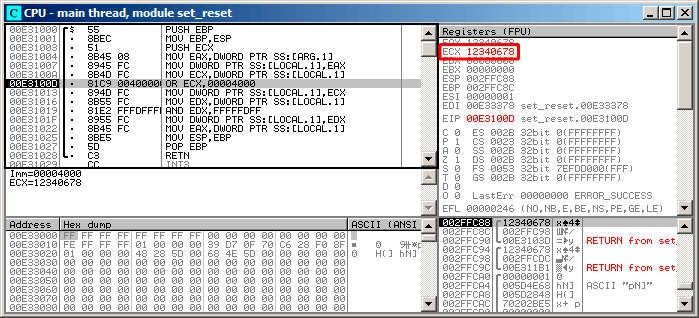
\includegraphics[scale=\FigScale]{patterns/14_bitfields/2_set_reset/olly1.png}
\caption{\olly: \EN{value is loaded into}\RU{значение загружено в} \ECX}
\label{fig:set_reset_olly1}
\end{figure}

\begin{figure}[H]
\centering
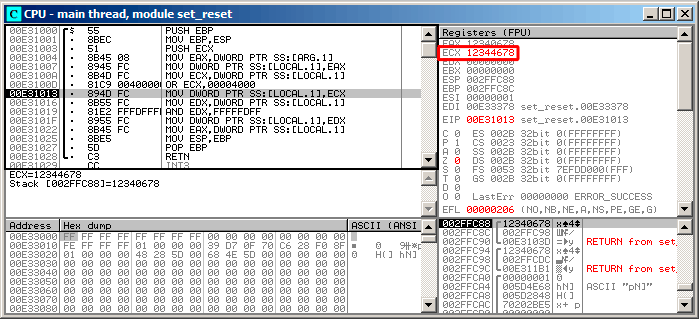
\includegraphics[scale=\FigScale]{patterns/14_bitfields/2_set_reset/olly2.png}
\caption{\olly: \OR \RU{сработал}\EN{executed}}
\label{fig:set_reset_olly2}
\end{figure}

\begin{figure}[H]
\centering
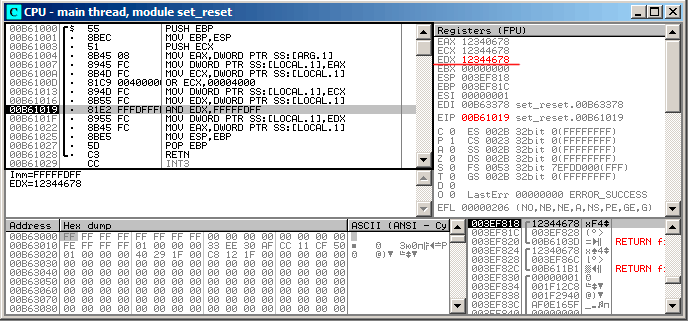
\includegraphics[scale=\FigScale]{patterns/14_bitfields/2_set_reset/olly3.png}
\caption{\olly: \EN{value was relaoded into}\RU{значение перезагрузилось в} \EDX}
\label{fig:set_reset_olly3}
\end{figure}

\begin{figure}[H]
\centering
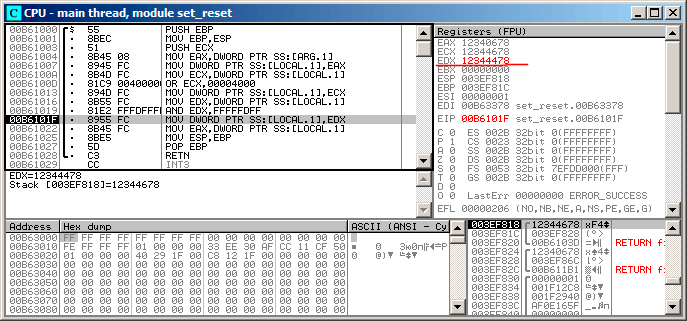
\includegraphics[scale=\FigScale]{patterns/14_bitfields/2_set_reset/olly4.png}
\caption{\olly: \ANDIns \RU{сработал}\EN{executed}}
\label{fig:set_reset_olly4}
\end{figure}

\subsubsection{\Optimizing MSVC}

\RU{Если скомпилировать в MSVC с оптимизацией (\Ox), то код будет еще короче:}
\EN{If we compile it in MSVC with optimization turned on (\Ox), the code will be even shorter:}

\lstinputlisting[caption=\Optimizing MSVC]{patterns/14_bitfields/2_set_reset/set_reset_msvc_Ox.asm}

\subsubsection{\NonOptimizing GCC}

\RU{Попробуем GCC 4.4.1 без оптимизации:}\EN{Let's try GCC 4.4.1 without optimization:}

\lstinputlisting[caption=\NonOptimizing GCC]{patterns/14_bitfields/2_set_reset/set_reset_gcc.asm}

\RU{Также избыточный код, хотя короче, чем у MSVC без оптимизации.}
\EN{There is a redundant code present,
however, it is shorter then MSVC version without optimization.}

\RU{Попробуем теперь GCC с оптимизацией}\EN{Now let's try GCC with optimization turned on} \Othree:

\subsubsection{\Optimizing GCC}

\lstinputlisting[caption=\Optimizing GCC]{patterns/14_bitfields/2_set_reset/set_reset_gcc_O3.asm}

\RU{Уже короче. Важно отметить что через регистр \AH, компилятор работает с частью регистра \EAX, 
эта его часть от 8-го до 15-го бита включительно.}
\EN{That's shorter.
It is worth noting the compiler works with the \EAX register part via the \AH 
register~---that is the \EAX register part from 8th to 15th bits inclusive.}

\RegTableOne{RAX}{EAX}{AX}{AH}{AL}

\index{x86!8086}
\index{x86!80386}
N.B. \RU{В 16-битном процессоре 8086 аккумулятор имел название \AX 
и состоял из двух 8-битных половин ~--- \AL (младшая часть) и \AH (старшая). 
В 80386 регистры были расширены до 32-бит, 
аккумулятор стал называться \EAX, но в целях совместимости, к его \IT{более старым} частям все еще можно 
обращаться как к \AX/\AH/\AL.}
\EN{16-bit CPU 8086 accumulator was named \AX and consisted of two 8-bit 
halves~---\AL (lower byte) and \AH (higher byte).
In 80386 almost all registers were extended to 32-bit, accumulator was named \EAX, 
but for the sake of compatibility,
its \IT{older parts} may be still accessed as \AX/\AH/\AL registers.}

\RU{Из-за того, что все x86 процессоры ~--- наследники 16-битного 8086, эти \IT{старые} 16-битные опкоды короче 
нежели более новые 32-битные. 
Поэтому, инструкция \TT{``or ah, 40h''} занимает только 3 байта. 
Было бы логичнее сгенерировать здесь \TT{``or eax, 04000h''}, но это уже 5 байт, или даже 6 
(если регистр в первом операнде не \EAX).}
\EN{Since all x86 CPUs are 16-bit 8086 CPU successors, these \IT{older} 16-bit opcodes are shorter 
than newer 32-bit opcodes.
That's why \TT{``or ah, 40h''} instruction occupying only 3 bytes.
It would be more logical way to emit here \TT{``or eax, 04000h''}
but that is 5 bytes, or even 6
(in case if register in first operand is not \EAX).}

\subsubsection{\Optimizing GCC \AndENRU regparm}

\RU{Если мы скомпилируем этот же пример не только с включенной оптимизацией \Othree, 
но еще и с опцией \TT{regparm=3}, о которой я писал немного выше, то получится еще короче:}
\EN{It would be even shorter if to turn on \Othree optimization flag and also set \TT{regparm=3}.}

\lstinputlisting[caption=\Optimizing GCC]{patterns/14_bitfields/2_set_reset/set_reset_gcc_O3_regparm3.asm}

\index{Inline code}
\RU{Действительно ~--- первый аргумент уже загружен в \EAX, и прямо здесь можно начинать с ним работать. 
Интересно, что и пролог функции (\TT{``push ebp / mov ebp,esp''}) и эпилог (\TT{``pop ebp''}) 
функции можно смело выкинуть
за ненадобностью, 
но возможно GCC еще не так хорош для подобных оптимизаций по размеру кода. 
Впрочем, в реальной жизни, подобные короткие функции лучше всего автоматически делать в виде 
\IT{inline-функций} (\ref{inline_code}).}
\EN{Indeed~---first argument is already loaded into \EAX, so it is possible to work with it in-place.
It is worth noting that both function prologue (\TT{``push ebp / mov ebp,esp''}) and epilogue (\TT{``pop ebp''})
can easily be omitted
here, but GCC probably is not good enough for such code size optimizations.
However, such short functions are better to be \IT{inlined functions} (\ref{inline_code}).}

\subsection{ARM + \OptimizingKeilVI (\ARMMode)}

\begin{lstlisting}[caption=\OptimizingKeilVI (\ARMMode)]
02 0C C0 E3          BIC     R0, R0, #0x200
01 09 80 E3          ORR     R0, R0, #0x4000
1E FF 2F E1          BX      LR
\end{lstlisting}

\index{ARM!\Instructions!BIC}
\TT{BIC} (\IT{BItwise bit Clear}) \RU{это инструкция сбрасывающая заданные биты. 
Это как аналог \TT{AND}, но только с инвертированным операндом.}\EN{is an instruction for clearing 
specific bits. This is just like the \TT{AND} instruction, but with inverted operand.}
\EN{I.e., it's analogous to a NOT+AND instruction pair.}
\RU{Т.е., это аналог инструкций NOT+AND.}

\index{ARM!\Instructions!ORR}
\TT{ORR} \RU{это \q{логическое или}, аналог}\EN{is \q{logical or}, analogous to} \OR \InENRU x86.

\RU{Пока всё понятно}\EN{So far it's easy}.

\subsection{ARM + \OptimizingKeilVI (\ThumbMode)}

\begin{lstlisting}[caption=\OptimizingKeilVI (\ThumbMode)]
01 21 89 03          MOVS    R1, 0x4000
08 43                ORRS    R0, R1
49 11                ASRS    R1, R1, #5   ; generate 0x200 and place to R1
88 43                BICS    R0, R1
70 47                BX      LR
\end{lstlisting}

\RU{Вероятно, Keil решил, что код в режиме thumb}
\EN{Seems like Keil decided that the code in thumb mode},
\RU{получающий}\EN{making} \TT{0x200} \RU{из}\EN{from} \TT{0x4000}, 
\RU{более компактный, нежели код,}\EN{is more compact than the code} 
\RU{записывающий}\EN{for writing} \TT{0x200} \RU{в какой-нибудь регистр}\EN{to an arbitrary register}.
% TODO1 пример, как компилятор при помощи сдвигов оптизирует такое: a=0x1000; b=0x2000; c=0x4000, etc

\index{ARM!\Instructions!ASRS}
\RU{Поэтому, при помощи инструкции}
\EN{So that is why, with the help of} \TT{ASRS} 
(\ASRdesc), \RU{это значение вычисляется как}\EN{this value is calculated as} $\TT{0x4000} \gg 5$.

\subsection{ARM + \OptimizingXcodeIV (\ARMMode)}
\label{anomaly:LLVM}
\index{\CompilerAnomaly}

\begin{lstlisting}[caption=\OptimizingXcodeIV (\ARMMode),label=ARM_leaf_example3]
42 0C C0 E3          BIC             R0, R0, #0x4200
01 09 80 E3          ORR             R0, R0, #0x4000
1E FF 2F E1          BX              LR
\end{lstlisting}

\RU{Код, который был сгенерирован LLVM, в исходном коде, на самом деле, выглядел бы так:}
\EN{The code that was generated by LLVM, in source code form could be something like this:}

\begin{lstlisting}
    REMOVE_BIT (rt, 0x4200);
    SET_BIT (rt, 0x4000);
\end{lstlisting}

\RU{И он делает то же самое что нам нужно}\EN{And it does exactly what we need}. 
\RU{Но почему}\EN{But why} \TT{0x4200}? 
\RU{Возможно, это артефакт оптимизатора LLVM}
\EN{Perhaps, that an artifact from LLVM's optimizer}
\footnote{\RU{Это был}\EN{It was} LLVM build 2410.2.00 \RU{входящий в состав}\EN{bundled with} Apple Xcode 4.6.3}.
\RU{Возможно, ошибка оптимизатора компилятора, но создаваемый код все же работает верно.}
\EN{Probably a compiler's optimizer error, but the generated code works correctly anyway.}

\RU{Об аномалиях компиляторов, подробнее читайте здесь}
\EN{You can read more about compiler anomalies here}~(\myref{anomaly:Intel}).

\OptimizingXcodeIV \RU{для режима Thumb генерирует точно такой же код.}
\EN{for thumb mode generates the same code.}

\subsection{ARM: \RU{еще об инструкции \TT{BIC}}\EN{more about the \TT{BIC} instruction}}
\index{ARM!\Instructions!BIC}

\RU{Если немного переделать пример}\EN{Let's rework the example slightly}:

\begin{lstlisting}
int f(int a)
{
    int rt=a;

    REMOVE_BIT (rt, 0x1234);

    return rt;
};
\end{lstlisting}

\EN{Then the optimizing}\RU{То оптимизирующий} Keil 5.03 
\RU{в режиме ARM сделает такое}\EN{in ARM mode does}:

\begin{lstlisting}
f PROC
        BIC      r0,r0,#0x1000
        BIC      r0,r0,#0x234
        BX       lr
        ENDP
\end{lstlisting}

\EN{There are two \TT{BIC} instructions, i.e., bit \TT{0x1234} are cleared in two passes.}
\RU{Здесь две инструкции \TT{BIC}, т.е. биты \TT{0x1234} сбрасываются в два прохода.}
\EN{This is because it's not possible to encode \TT{0x1234} in a \TT{BIC} instruction, 
but it's possible to encode \TT{0x1000} and \TT{0x234}.}
\RU{Это потому что в инструкции \TT{BIC} нельзя закодировать самое значение \TT{0x1234}, 
но можно закодировать \TT{0x1000} либо \TT{0x234}.}

\subsection{ARM64: \Optimizing GCC (Linaro) 4.9}

\Optimizing GCC \RU{компилирующий для ARM64 может использовать \TT{AND} вместо}\EN{compiling for ARM64 can use 
the \TT{AND} instruction instead of} \TT{BIC}:

\begin{lstlisting}[caption=\Optimizing GCC (Linaro) 4.9]
f:
	and	w0, w0, -513	; 0xFFFFFFFFFFFFFDFF
	orr	w0, w0, 16384	; 0x4000
	ret
\end{lstlisting}

\subsection{ARM64: \NonOptimizing GCC (Linaro) 4.9}

\NonOptimizing GCC \RU{генерирует больше избыточного кода, но он работает также}\EN{generates more redundant 
code, but works just like optimized}:

\begin{lstlisting}[caption=\NonOptimizing GCC (Linaro) 4.9]
f:
	sub	sp, sp, #32
	str	w0, [sp,12]
	ldr	w0, [sp,12]
	str	w0, [sp,28]
	ldr	w0, [sp,28]
	orr	w0, w0, 16384	; 0x4000
	str	w0, [sp,28]
	ldr	w0, [sp,28]
	and	w0, w0, -513	; 0xFFFFFFFFFFFFFDFF
	str	w0, [sp,28]
	ldr	w0, [sp,28]
	add	sp, sp, 32
	ret
\end{lstlisting}



\section{\ShiftsSectionName}

\RU{Битовые сдвиги в \CCpp реализованы при помощи операторов $\ll$ и $\gg$.}
\EN{Bit shifts in \CCpp are implemented via $\ll$ and $\gg$ operators.}

\RU{В x86 есть инструкции}\EN{x86 \ac{ISA} has} SHL (SHift Left) \AndENRU SHR (SHift Right) 
\RU{для этого}\EN{instructions for this}.

\subsection{\RU{Деление и умножение при помощи сдвигов}\EN{Division and multiplication using shifts}}
\label{subsec:mult_div_shifts}

\RU{Инструкции сдвига также активно применяются при делении или умножении 
на числа-степени двойки: $2^{n}$ (т.е., $1$, $2$, $4$, $8$, и т.д.).}
\EN{Shift instructions are often used in division and multiplications by power of two numbers:
$2^{n}$ (e.g., $1$, $2$, $4$, $8$, etc).}

\subsubsection{\RU{Умножение}\EN{Multiplication}}

\begin{lstlisting}
unsigned int f(unsigned int a)
{
	return a*4;
};
\end{lstlisting}

\begin{lstlisting}[caption=\NonOptimizing MSVC 2010]
_a$ = 8		; size = 4
_f	PROC
	push	ebp
	mov	ebp, esp
	mov	eax, DWORD PTR _a$[ebp]
	shl	eax, 2
	pop	ebp
	ret	0
_f	ENDP
\end{lstlisting}

\RU{Умножить на $4$ это просто сдвинуть число на 2 бита влево, 
вставив 2 нулевых бита справа (как два самых младших бита). 
Это как умножить $3$ на $100$ ~--- нужно просто дописать два нуля справа.}
\EN{Multiplication by $4$ is just shifting the number to the left by 2 bits,
while inserting 2 zero bits at right (as the last two bits).
It is just like to multiply $3$ by $100$~---we need just to add two zeroes at the right.}

\RU{Вот как работает инструкция сдвига влево}\EN{That's how shift left instruction works}:

\index{x86!\Instructions!SHL}
\begin{center}
	\begin{tikzpicture}[scale=0.7, every node/.style={scale=0.7}]
	\edef\bitsize{1cm}
	\tikzstyle{byte}=[draw,minimum size=\bitsize]	
	\tikzstyle{every path}=[thick]

	\node [draw,rectangle,minimum size=\bitsize] (a1) {7};
	\node [draw,rectangle,minimum size=\bitsize] (a2) [right of=a1] {6};
	\node [draw,rectangle,minimum size=\bitsize] (a3) [right of=a2] {5};
	\node [draw,rectangle,minimum size=\bitsize] (a4) [right of=a3] {4};
	\node [draw,rectangle,minimum size=\bitsize] (a5) [right of=a4] {3};
	\node [draw,rectangle,minimum size=\bitsize] (a6) [right of=a5] {2};
	\node [draw,rectangle,minimum size=\bitsize] (a7) [right of=a6] {1};
	\node [draw,rectangle,minimum size=\bitsize] (a8) [right of=a7] {0};

	\node (empty) [below of=a1] {};

	\node [draw,rectangle,minimum size=\bitsize] (b1) [below of=empty] {7};
	\node [draw,rectangle,minimum size=\bitsize] (b2) [right of=b1] {6};
	\node [draw,rectangle,minimum size=\bitsize] (b3) [right of=b2] {5};
	\node [draw,rectangle,minimum size=\bitsize] (b4) [right of=b3] {4};
	\node [draw,rectangle,minimum size=\bitsize] (b5) [right of=b4] {3};
	\node [draw,rectangle,minimum size=\bitsize] (b6) [right of=b5] {2};
	\node [draw,rectangle,minimum size=\bitsize] (b7) [right of=b6] {1};
	\node [draw,rectangle,minimum size=\bitsize] (b8) [right of=b7] {0};
	
	\node [shape=rectangle,draw,minimum size=\bitsize] (d) [left=of b1] {nowhere};
	\node [shape=rectangle,draw,minimum size=\bitsize] (c) [right=of b8] {0};
	
	\draw [->] (c.west) -- (b8.east);

	\draw [->] (a2.south) -- (b1.north);
	\draw [->] (a3.south) -- (b2.north);
	\draw [->] (a4.south) -- (b3.north);
	\draw [->] (a5.south) -- (b4.north);
	\draw [->] (a6.south) -- (b5.north);
	\draw [->] (a7.south) -- (b6.north);
	\draw [->] (a8.south) -- (b7.north);
	
	\draw [->] (a1.south) -- (d.north);

	\end{tikzpicture}
\end{center}


\RU{Добавленные биты справа --- всегда нули}\EN{Added bits at right---always zeroes}.

\RU{Умножение на 4 в}\EN{Multiplication by 4 in} ARM:

\begin{lstlisting}[caption=\NonOptimizingKeilVI + \ARMMode]
f PROC
        LSL      r0,r0,#2
        BX       lr
        ENDP
\end{lstlisting}

\subsubsection{\RU{Деление}\EN{Division}}

\RU{Например}\EN{For example}:

\begin{lstlisting}
unsigned int f(unsigned int a)
{
	return a/4;
};
\end{lstlisting}

\RU{Имеем в итоге}\EN{We got} (MSVC 2010):

\begin{lstlisting}[caption=MSVC 2010]
_a$ = 8							; size = 4
_f	PROC
	mov	eax, DWORD PTR _a$[esp-4]
	shr	eax, 2
	ret	0
_f	ENDP
\end{lstlisting}

\label{SHR}
\index{x86!\Instructions!SHR}
\RU{Инструкция \SHR (\IT{SHift Right}) в данном примере сдвигает число на 2 бита вправо. 
При этом, освободившиеся два бита слева (т.е., самые 
старшие разряды), выставляются в нули. А самые младшие 2 бита выкидываются. 
Фактически, эти два выкинутых бита ~--- остаток от деления.}
\EN{\SHR (\IT{SHift Right}) instruction in this example is shifting a number by 2 bits right.
Two freed bits at left (e.g., two most significant bits) are set to zero.
Two least significant bits are dropped.
In fact, these two dropped bits~---division operation remainder.}

\index{x86!\Instructions!SHR}
\RU{Инструкция \SHR работает так же, как и \SHL, только в другую сторону.}
\EN{\SHR instruction works just like as \SHL but in other direction.}

\begin{center}
	\begin{tikzpicture}[scale=0.7, every node/.style={scale=0.7}]
	\edef\bitsize{1cm}
	\tikzstyle{byte}=[draw,minimum size=\bitsize]	
	\tikzstyle{every path}=[thick]

	\node [draw,rectangle,minimum size=\bitsize] (a1) {7};
	\node [draw,rectangle,minimum size=\bitsize] (a2) [right of=a1] {6};
	\node [draw,rectangle,minimum size=\bitsize] (a3) [right of=a2] {5};
	\node [draw,rectangle,minimum size=\bitsize] (a4) [right of=a3] {4};
	\node [draw,rectangle,minimum size=\bitsize] (a5) [right of=a4] {3};
	\node [draw,rectangle,minimum size=\bitsize] (a6) [right of=a5] {2};
	\node [draw,rectangle,minimum size=\bitsize] (a7) [right of=a6] {1};
	\node [draw,rectangle,minimum size=\bitsize] (a8) [right of=a7] {0};

	\node (empty) [below of=a1] {};

	\node [draw,rectangle,minimum size=\bitsize] (b1) [below of=empty] {7};
	\node [draw,rectangle,minimum size=\bitsize] (b2) [right of=b1] {6};
	\node [draw,rectangle,minimum size=\bitsize] (b3) [right of=b2] {5};
	\node [draw,rectangle,minimum size=\bitsize] (b4) [right of=b3] {4};
	\node [draw,rectangle,minimum size=\bitsize] (b5) [right of=b4] {3};
	\node [draw,rectangle,minimum size=\bitsize] (b6) [right of=b5] {2};
	\node [draw,rectangle,minimum size=\bitsize] (b7) [right of=b6] {1};
	\node [draw,rectangle,minimum size=\bitsize] (b8) [right of=b7] {0};
	
	\node [shape=rectangle,draw,minimum size=\bitsize] (c) [left=of b1] {0};
	\node [shape=rectangle,draw,minimum size=\bitsize] (d) [right=of b8] {CF};
	
	\draw [->] (c.east) -- (b1.west);

	\draw [->] (a1.south) -- (b2.north);
	\draw [->] (a2.south) -- (b3.north);
	\draw [->] (a3.south) -- (b4.north);
	\draw [->] (a4.south) -- (b5.north);
	\draw [->] (a5.south) -- (b6.north);
	\draw [->] (a6.south) -- (b7.north);
	\draw [->] (a7.south) -- (b8.north);
	
	\draw [->] (a8.south) -- (d.north);

	\end{tikzpicture}
\end{center}



\label{division_by_shifting}
\RU{Для того, чтобы это проще понять, представьте себе десятичную систему счисления и число $23$. 
$23$ можно разделить на $10$ просто откинув последний разряд ($3$ ~--- это остаток от деления). 
После этой операции останется $2$ как \glslink{quotient}{частное}.}
\EN{It can be easily understood if to imagine decimal numeral system and number $23$.
$23$ can be easily divided by $10$ just by dropping last digit ($3$~---is division remainder). 
$2$ is leaving after operation as a \gls{quotient}.}

\RU{Деление на 4 в}\EN{Division by 4 in} ARM:

\begin{lstlisting}[caption=\NonOptimizingKeilVI + \ARMMode]
f PROC
        LSR      r0,r0,#2
        BX       lr
        ENDP
\end{lstlisting}

\subsection{\RU{Подсчет выставленных бит}\EN{Counting bits set to 1}}

\RU{Вот этот несложный пример иллюстрирует функцию, считающую количество бит-единиц во входной переменной.}
\EN{Here is a simple example of function, calculating number of $1$ bits in input variable.}

\RU{Эта ф-ция также называется}\EN{This function is also called} ``population count''
\footnote{\RU{современные x86-процессоры (поддерживающие SSE4) даже имеют инструкцию POPCNT для этого}
\EN{modern x86 CPUs (supporting SSE4) even have POPCNT instruction for it}}.

\lstinputlisting{patterns/14_bitfields/3_shifts/shifts.c}

\RU{В этом цикле, счетчик итераций \IT{i} считает от $0$ до $31$, а $1 \ll i$ будет от $1$ до \TT{0x80000000}. 
Описывая это словами, можно сказать 
\IT{сдвинуть единицу на $n$ бит влево}.
Т.е., в некотором смысле, выражение $1 \ll i$ последовательно выдаст все возможные позиции бит в 32-битном числе. 
Кстати, освободившийся бит справа всегда обнуляется.}
\EN{In this loop, iteration count value \IT{i} counting from $0$ to $31$, $1 \ll i$ statement will be counting 
from $1$ to \TT{0x80000000}.
Describing this operation in natural language, we would say \IT{shift $1$ by n bits left}.
In other words, $1 \ll i$ statement will consequently produce all possible bit positions in 32-bit number.
By the way, freed bit at right is always cleared.}

\RU{Вот таблица всех возможных значений}\EN{Here is a table of all possible} $1 \ll i$ 
\RU{для}\EN{for} $i=0 \ldots 31$:

\begin{center}
\begin{tabular}{ | l | l | l | l | }
\hline
\cellcolor{blue!25} \RU{Выражение в }\CCpp\EN{ expression} & 
\cellcolor{blue!25} \RU{Степень двойки}\EN{Power of two} & 
\cellcolor{blue!25} \RU{Десятичная форма}\EN{Decimal form} & 
\cellcolor{blue!25} \RU{Шестнадцатеричная форма}\EN{Hexadecimal form} \\
\hline
$1 \ll 0$ & 1 & 1 & 1 \\
\hline
$1 \ll 1$ & $2^{1}$ & 2 & 2 \\
\hline
$1 \ll 2$ & $2^{2}$ & 4 & 4 \\
\hline
$1 \ll 3$ & $2^{3}$ & 8 & 8 \\
\hline
$1 \ll 4$ & $2^{4}$ & 16 & 0x10 \\
\hline
$1 \ll 5$ & $2^{5}$ & 32 & 0x20 \\
\hline
$1 \ll 6$ & $2^{6}$ & 64 & 0x40 \\
\hline
$1 \ll 7$ & $2^{7}$ & 128 & 0x80 \\
\hline
$1 \ll 8$ & $2^{8}$ & 256 & 0x100 \\
\hline
$1 \ll 9$ & $2^{9}$ & 512 & 0x200 \\
\hline
$1 \ll 10$ & $2^{10}$ & 1024 & 0x400 \\
\hline
$1 \ll 11$ & $2^{11}$ & 2048 & 0x800 \\
\hline
$1 \ll 12$ & $2^{12}$ & 4096 & 0x1000 \\
\hline
$1 \ll 13$ & $2^{13}$ & 8192 & 0x2000 \\
\hline
$1 \ll 14$ & $2^{14}$ & 16384 & 0x4000 \\
\hline
$1 \ll 15$ & $2^{15}$ & 32768 & 0x8000 \\
\hline
$1 \ll 16$ & $2^{16}$ & 65536 & 0x10000 \\
\hline
$1 \ll 17$ & $2^{17}$ & 131072 & 0x20000 \\
\hline
$1 \ll 18$ & $2^{18}$ & 262144 & 0x40000 \\
\hline
$1 \ll 19$ & $2^{19}$ & 524288 & 0x80000 \\
\hline
$1 \ll 20$ & $2^{20}$ & 1048576 & 0x100000 \\
\hline
$1 \ll 21$ & $2^{21}$ & 2097152 & 0x200000 \\
\hline
$1 \ll 22$ & $2^{22}$ & 4194304 & 0x400000 \\
\hline
$1 \ll 23$ & $2^{23}$ & 8388608 & 0x800000 \\
\hline
$1 \ll 24$ & $2^{24}$ & 16777216 & 0x1000000 \\
\hline
$1 \ll 25$ & $2^{25}$ & 33554432 & 0x2000000 \\
\hline
$1 \ll 26$ & $2^{26}$ & 67108864 & 0x4000000 \\
\hline
$1 \ll 27$ & $2^{27}$ & 134217728 & 0x8000000 \\
\hline
$1 \ll 28$ & $2^{28}$ & 268435456 & 0x10000000 \\
\hline
$1 \ll 29$ & $2^{29}$ & 536870912 & 0x20000000 \\
\hline
$1 \ll 30$ & $2^{30}$ & 1073741824 & 0x40000000 \\
\hline
$1 \ll 31$ & $2^{31}$ & 2147483648 & 0x80000000 \\
\hline
\end{tabular}
\end{center}

\RU{Это числа-константы (битовые маски), которые крайне часто попадаются в практике reverse engineer-а, и их нужно
уметь распозновать.}
\EN{These constant numbers (bit masks) are very often appears in code and practicing reverse engineer should quickly
to spot them.}
\RU{Числа в десятичном виде заучивать, пожалуй, незачем, а числа в шестнадцатиричном
виде итак легко запомнить.}
\EN{You probably shouldn't memorize decimal numbers, but hexadecimal ones are very easy to remember.}

\RU{Эти константы очень часто используются для определения отдельных бит как флагов.}
\EN{These constants are very often used for mapping flags to specific bits.}
\RU{Например, это из файла}\EN{For example, here is excerpt from} \TT{ssl\_private.h} \RU{из исходников}
\EN{file from} Apache 2.4.6\EN{ source code}:

\begin{lstlisting}
/**
 * Define the SSL options
 */
#define SSL_OPT_NONE           (0)
#define SSL_OPT_RELSET         (1<<0)
#define SSL_OPT_STDENVVARS     (1<<1)
#define SSL_OPT_EXPORTCERTDATA (1<<3)
#define SSL_OPT_FAKEBASICAUTH  (1<<4)
#define SSL_OPT_STRICTREQUIRE  (1<<5)
#define SSL_OPT_OPTRENEGOTIATE (1<<6)
#define SSL_OPT_LEGACYDNFORMAT (1<<7)
\end{lstlisting}

\RU{Вернемся назад к нашему примеру}\EN{Let's back to our example}.

\RU{Макрос \TT{IS\_SET} проверяет наличие этого бита в \TT{a}.}
\EN{\TT{IS\_SET} macro is checking bit presence in the \TT{a}.}

\index{x86!\Instructions!AND}
\RU{Макрос \TT{IS\_SET} на самом деле это операция логического И (\IT{AND}) 
и она возвращает $0$ если бита там нет, 
либо эту же битовую маску, если бит там есть. 
В \CCpp, конструкция \TT{if()} срабатывает, если выражение внутри её не ноль, пусть хоть $123456$, 
поэтому все будет работать.}
\EN{The \TT{IS\_SET} macro is in fact logical and operation (\IT{AND}) 
and it returns $0$ if specific bit is absent there,
or bit mask, if the bit is present.
\IT{if()} operator triggered in \CCpp if expression in it is not a zero, it might be even $123456$, that is why
it always working correctly.}

% subsubsections
\subsection{x86}

\RU{Компилируем}\EN{Let's compile} (MSVC 2010):

\lstinputlisting[caption=MSVC 2010]{patterns/14_bitfields/3_shifts/shifts_MSVC_\LANG.asm}

\RU{Вот так работает SHL (\IT{SHift Left})}
\EN{That's how SHL (\IT{SHift Left}) working}.

\RU{Скомпилируем то же и в}\EN{Let's compile it in} GCC 4.4.1:

\lstinputlisting[caption=GCC 4.4.1]{patterns/14_bitfields/3_shifts/shifts_gcc.asm}

\RU{Инструкции сдвига также активно применяются при делении или умножении 
на числа-степени двойки ($1$, $2$, $4$, $8$, и т.д.).}
\EN{Shift instructions are often used in division and multiplications by power of two numbers 
($1$, $2$, $4$, $8$, etc).}

\RU{Например}\EN{For example}:

\begin{lstlisting}
unsigned int f(unsigned int a)
{
	return a/4;
};
\end{lstlisting}

\RU{Имеем в итоге}\EN{We got} (MSVC 2010):

\begin{lstlisting}[caption=MSVC 2010]
_a$ = 8							; size = 4
_f	PROC
	mov	eax, DWORD PTR _a$[esp-4]
	shr	eax, 2
	ret	0
_f	ENDP
\end{lstlisting}

\label{SHR}
\index{x86!\Instructions!SHR}
\RU{Инструкция \SHR (\IT{SHift Right}) в данном примере сдвигает число на 2 бита вправо. 
При этом, освободившиеся два бита слева (т.е., самые 
старшие разряды), выставляются в нули. А самые младшие 2 бита выкидываются. 
Фактически, эти два выкинутых бита ~--- остаток от деления.}
\EN{\SHR (\IT{SHift Right}) instruction in this example is shifting a number by 2 bits right.
Two freed bits at left (e.g., two most significant bits) are set to zero.
Two least significant bits are dropped.
In fact, these two dropped bits~---division operation remainder.}

\index{x86!\Instructions!SHR}
\RU{Инструкция \SHR работает так же, как и \SHL, только в другую сторону.}
\EN{\SHR instruction works just like as \SHL but in other direction.}

\begin{center}
	\begin{tikzpicture}[scale=0.7, every node/.style={scale=0.7}]
	\edef\bitsize{1cm}
	\tikzstyle{byte}=[draw,minimum size=\bitsize]	
	\tikzstyle{every path}=[thick]

	\node [draw,rectangle,minimum size=\bitsize] (a1) {7};
	\node [draw,rectangle,minimum size=\bitsize] (a2) [right of=a1] {6};
	\node [draw,rectangle,minimum size=\bitsize] (a3) [right of=a2] {5};
	\node [draw,rectangle,minimum size=\bitsize] (a4) [right of=a3] {4};
	\node [draw,rectangle,minimum size=\bitsize] (a5) [right of=a4] {3};
	\node [draw,rectangle,minimum size=\bitsize] (a6) [right of=a5] {2};
	\node [draw,rectangle,minimum size=\bitsize] (a7) [right of=a6] {1};
	\node [draw,rectangle,minimum size=\bitsize] (a8) [right of=a7] {0};

	\node (empty) [below of=a1] {};

	\node [draw,rectangle,minimum size=\bitsize] (b1) [below of=empty] {7};
	\node [draw,rectangle,minimum size=\bitsize] (b2) [right of=b1] {6};
	\node [draw,rectangle,minimum size=\bitsize] (b3) [right of=b2] {5};
	\node [draw,rectangle,minimum size=\bitsize] (b4) [right of=b3] {4};
	\node [draw,rectangle,minimum size=\bitsize] (b5) [right of=b4] {3};
	\node [draw,rectangle,minimum size=\bitsize] (b6) [right of=b5] {2};
	\node [draw,rectangle,minimum size=\bitsize] (b7) [right of=b6] {1};
	\node [draw,rectangle,minimum size=\bitsize] (b8) [right of=b7] {0};
	
	\node [shape=rectangle,draw,minimum size=\bitsize] (c) [left=of b1] {0};
	\node [shape=rectangle,draw,minimum size=\bitsize] (d) [right=of b8] {CF};
	
	\draw [->] (c.east) -- (b1.west);

	\draw [->] (a1.south) -- (b2.north);
	\draw [->] (a2.south) -- (b3.north);
	\draw [->] (a3.south) -- (b4.north);
	\draw [->] (a4.south) -- (b5.north);
	\draw [->] (a5.south) -- (b6.north);
	\draw [->] (a6.south) -- (b7.north);
	\draw [->] (a7.south) -- (b8.north);
	
	\draw [->] (a8.south) -- (d.north);

	\end{tikzpicture}
\end{center}



\label{division_by_shifting}
\RU{Для того, чтобы это проще понять, представьте себе десятичную систему счисления и число $23$. 
$23$ можно разделить на $10$ просто откинув последний разряд ($3$ ~--- это остаток от деления). 
После этой операции останется $2$ как \glslink{quotient}{частное}.}
\EN{It can be easily understood if to imagine decimal numeral system and number $23$.
$23$ can be easily divided by $10$ just by dropping last digit ($3$~---is division remainder). 
$2$ is leaving after operation as a \gls{quotient}.}

\RU{Так и с умножением. Умножить на $4$ это просто сдвинуть число на 2 бита влево, 
вставив 2 нулевых бита справа (как два самых младших бита). 
Это как умножить $3$ на $100$ ~--- нужно просто дописать два нуля справа.}
\EN{The same story about multiplication.
Multiplication by $4$ is just shifting the number to the left by 2 bits,
while inserting 2 zero bits at right (as the last two bits).
It is just like to multiply $3$ by $100$~---we need just to add two zeroes at the right.}



\subsubsection{ARM + \OptimizingXcode + \ARMMode}

\begin{lstlisting}[caption=\OptimizingXcode + \ARMMode]
                MOV             R1, R0
                MOV             R0, #0
                MOV             R2, #1
                MOV             R3, R0
loc_2E54
                TST             R1, R2,LSL R3 ; set flags according to R1 & (R2<<R3)
                ADD             R3, R3, #1    ; R3++
                ADDNE           R0, R0, #1    ; if ZF flag is cleared by TST, R0++
                CMP             R3, #32
                BNE             loc_2E54
                BX              LR
\end{lstlisting}

\index{ARM!\Instructions!TST}
\TT{TST} \RU{это то же что и}\EN{is the same things as} \TEST \InENRU x86.

\index{ARM!Optional operators!LSL}
\index{ARM!Optional operators!LSR}
\index{ARM!Optional operators!ASR}
\index{ARM!Optional operators!ROR}
\index{ARM!Optional operators!RRX}
\index{ARM!\Instructions!MOV}
\index{ARM!\Instructions!TST}
\index{ARM!\Instructions!CMP}
\index{ARM!\Instructions!ADD}
\index{ARM!\Instructions!SUB}
\index{ARM!\Instructions!RSB}
\RU{Как я уже указывал}\EN{As I mentioned before}~(\ref{shifts_in_ARM_mode}),
\RU{в режиме ARM нет отдельной инструкции для сдвигов.}
\EN{there are no separate shifting instructions in ARM mode.}
\RU{Однако, модификаторами}\EN{However, there are modifiers} 
LSL (\IT{Logical Shift Left}), 
LSR (\IT{Logical Shift Right}), 
ASR (\IT{Arithmetic Shift Right}), 
ROR (\IT{Rotate Right}) \AndENRU 
RRX (\IT{Rotate Right with Extend}) \RU{можно дополнять некоторые инструкции, такие как}
\EN{, which may be added to such instructions as} \MOV, \TT{TST},
\CMP, \ADD, \SUB, \TT{RSB}\footnote{\DataProcessingInstructionsFootNote}.

\RU{Эти модификаторы указывают, как сдвигать второй операнд, и на сколько.}
\EN{These modificators are defines, how to shift second operand and by how many bits.}

\index{ARM!Optional operators!LSL}
\RU{Таким образом, инструкция }\EN{Thus} \TT{``TST R1, R2,LSL R3''} 
\RU{здесь работает как}\EN{instruction works here as} $R1 \land (R2 \ll R3)$.

\subsubsection{ARM + \OptimizingXcode + \ThumbTwoMode}

\index{ARM!\Instructions!LSL.W}
\index{ARM!\Instructions!LSL}
\RU{Почти такое же}\EN{Almost the same}, 
\RU{только здесь применяется пара инструкций}\EN{but here are two} 
\TT{LSL.W}/\TT{TST} 
\RU{вместо одной}\EN{instructions are used instead of single} 
\TT{TST},
\RU{ведь в режиме thumb нельзя добавлять указывать модификатор}\EN{because, in thumb mode, it is not
possible to define} \TT{LSL} \RU{прямо в}\EN{modifier right in} \TT{TST}.

\begin{lstlisting}
                MOV             R1, R0
                MOVS            R0, #0
                MOV.W           R9, #1
                MOVS            R3, #0
loc_2F7A
                LSL.W           R2, R9, R3
                TST             R2, R1
                ADD.W           R3, R3, #1
                IT NE
                ADDNE           R0, #1
                CMP             R3, #32
                BNE             loc_2F7A
                BX              LR
\end{lstlisting}



\section{\RU{Установка и сброс отдельного бита: пример с \ac{FPU}}\EN{Setting and clearing specific bits: \ac{FPU} example}}

\index{IEEE 754}
\RU{Как мы уже можем знать, вот как биты расположены в значении типа \Tfloat в формате IEEE 754:}
\EN{Here is how bits are located in the \Tfloat type in IEEE 754 form:}

\bigskip
% a hack used here! http://tex.stackexchange.com/questions/73524/bytefield-package
\begin{center}
\begin{bytefield}{32}
	\bitheader[endianness=big]{0,22,23,30,31} \\
	\bitbox{1}{S} & 
	\bitbox{8}{%
		\RU{экспонента}%
		\EN{exponent}%
		\ES{exponente}%
		\PTBRph{}%
		\DEph{}\PLph{}%
		\ITAph{}%
		\FR{exposant}
	} & 
	\bitbox{23}{%
		\RU{мантисса}%
		\EN{mantissa or fraction}%
		\ES{mantisa o fracci\'on}%
		\PTBRph{}%
		\DEph{}\PLph{}%
		\ITAph{}%
		\FR{mantisse ou fraction}
	}
\end{bytefield}
\end{center}

\begin{center}
( S\EMDASH{}%
	\RU{знак}%
	\EN{sign}%
	\ES{signo}%
	\PTBRph{}%
	\DEph{}\PLph{}%
	\ITAph{}%
	\FR{signe}
)
\end{center}


\RU{Знак числа~--- это}\EN{The sign of number is in the} \ac{MSB}. 
\RU{Возможно ли работать со знаком числа с плавающей точкой, не используя FPU-инструкций?}
\EN{Will it be possible to change the sign of a floating point number without any FPU instructions?}

\lstinputlisting{patterns/14_bitfields/35_set_reset_FPU/abs.c}

\RU{Придется использовать эти трюки в \CCpp с типами данных чтобы копировать из значения типа \Tfloat и обратно
без конверсии.}
\EN{We need this trickery in \CCpp to copy to/from \Tfloat value without actual conversion.}
\RU{Так что здесь три функции: my\_abs() сбрасывает \ac{MSB}; set\_sign() устанавливает \ac{MSB} и 
negate() меняет его на противоположный.}
\EN{So there are three functions: my\_abs() resets \ac{MSB}; set\_sign() sets \ac{MSB} and negate() flips it.}

\subsection{\RU{Кое-что об операции \XOR}\EN{A word about the \XOR operation}}

% included twice... a bit of redundancy, but it's OK

\RU{\XOR (исключающее ИЛИ) часто используется для того чтобы поменять какой-то бит(ы) на противоположный.}
\EN{\XOR is widely used when one need just to flip specific bit(s).}
\RU{Действительно, операция \XOR с 1 на самом деле просто инвертирует бит:}
\EN{Indeed, the \XOR operation applied with 1 is effectively inverting a bit:}

\begin{center}
\begin{tabular}{ | l | l | l | }
\hline
\cellcolor{blue!25} \RU{вход А}\EN{input A} & 
\cellcolor{blue!25} \RU{вход Б}\EN{input B} & 
\cellcolor{blue!25} \RU{выход}\EN{output} \\
\hline
0 & 0 & 0 \\
\hline
{\color{red} 0} & {\color{red} 1} & {\color{red} 1} \\
\hline
{\color{red} 1} & {\color{red} 0} & {\color{red} 1} \\
\hline
1 & 1 & 0 \\
\hline
\end{tabular}
\end{center}

\RU{И наоборот, операция \XOR с 0 ничего не делает, т.е. это холостая операция.}
\EN{And on the contrary, the \XOR operation applied with 0 does nothing, i.e., it's an idle operation.}
\RU{Это очень важное свойство операции \XOR и очень важно помнить его.}
\EN{This is a very important property of the \XOR operation and it's highly recommended to memorize it.}


\subsection{x86}

\RU{Код прямолинеен}\EN{The code is pretty straightforward}:

\lstinputlisting[caption=\Optimizing MSVC 2012]{patterns/14_bitfields/35_set_reset_FPU/abs_MSVC2012_Ox.asm}

\RU{Входное значение типа \Tfloat берется из стека, но мы обходимся с ним как с целочисленным значением.}
\EN{An input value of type \Tfloat is taken from the stack, but treated as an integer value.}

\AND \AndENRU \OR \RU{сбрасывают и устанавливают нужный бит}\EN{reset and set the desired bit}.
\XOR \RU{переворачивает его}\EN{flips it}.

\RU{В конце измененное значение загружается в ST0, потому что числа с плавающей точкой возвращаются в этом 
регистре.}
\EN{Finally, the modified value is loaded into ST0, because floating-point numbers are returned in this register.}

\RU{Попробуем оптимизирующий MSVC 2012 для x64}\EN{Now let's try optimizing MSVC 2012 for x64}:

\lstinputlisting[caption=\Optimizing MSVC 2012 x64]{patterns/14_bitfields/35_set_reset_FPU/abs_MSVC2012_x64_Ox.asm}

\index{x86!\Instructions!BTR}
\index{x86!\Instructions!BTS}
\index{x86!\Instructions!BTC}
\RU{Во-первых, входное значение передается в XMM0, затем оно копируется в локальный стек и затем мы видим
новые для нас инструкции: \BTR, \BTS, \BTC.}
\EN{The input value is passed in XMM0, then it is copied into the local stack and then we see 
some instructions that are new to us: \BTR, \BTS, \BTC.}

\RU{Эти инструкции используются для сброса определенного бита (\BTR: \q{reset}), 
установки (\BTS: \q{set}) и инвертирования (\BTC: \q{complement}).}
\EN{These instructions are used for resetting (\BTR), setting (\BTS) and inverting (or complementing: \BTC) 
specific bits.}
\RU{31-й бит это \ac{MSB}, если считать с нуля}\EN{The 31st bit is \ac{MSB}, counting from 0}.

\RU{И наконец, результат копируется в регистр XMM0, потому что значения с плавающей точной возвращаются
в регистре XMM0 в среде Win64.}
\EN{Finally, the result is copied into XMM0, because floating point values are returned through XMM0 in Win64
environment.}

\ifdefined\IncludeMIPS
\subsection{MIPS}

GCC 4.4.5 \ForENRU MIPS \RU{делает почти то же самое}\EN{does mostly the same}:

\lstinputlisting[caption=\Optimizing GCC 4.4.5 (IDA)]{patterns/14_bitfields/35_set_reset_FPU/MIPS_O3_IDA.lst.\LANG}

\index{MIPS!\Instructions!LUI}
\RU{Для загрузки константы 0x80000000 в регистр используется только одна инструкция \LUI, потому что \LUI сбрасывает
младшие 16 бит и это нули в константе, так что одной \LUI без \ORI достаточно.}
\EN{One single \LUI instruction is used to load 0x80000000 into a register, because 
\LUI is clearing the low 16 bits and these are zeroes in the constant, so one \LUI without subsequent \ORI is enough.}

\fi

\ifdefined\IncludeARM
\subsection{ARM}

\subsubsection{\OptimizingKeilVI (\ARMMode)}

\lstinputlisting[caption=\OptimizingKeilVI (\ARMMode)]{patterns/14_bitfields/35_set_reset_FPU/abs_Keil_ARM_O3.s.\LANG}

\RU{Пока всё понятно}\EN{So far so good}.
\index{ARM!\Instructions!BIC}
\index{ARM!\Instructions!EOR}
\RU{В ARM есть инструкция \BIC для сброса заданных бит.}
\EN{ARM has the \BIC instruction, which explicitly clears specific bit(s).}
\RU{\EOR это инструкция в ARM которая делает то же что и \XOR}\EN{\EOR is the ARM instruction name for \XOR} 
(\q{Exclusive OR}).

\subsubsection{\OptimizingKeilVI (\ThumbMode)}

\lstinputlisting[caption=\OptimizingKeilVI (\ThumbMode)]{patterns/14_bitfields/35_set_reset_FPU/abs_Keil_thumb_O3.s}

\RU{В режиме Thumb 16-битные инструкции, в которых нельзя задать много данных, поэтому здесь
применяется пара инструкций \MOVS/\LSLS для формирования константы 0x80000000.}
\EN{Thumb mode in ARM offers 16-bit instructions and not much data can be encoded in them, so here a 
MOVS/LSLS instruction pair is used for forming the 0x80000000 constant.}
\RU{Это работает как выражение}\EN{It works like this}: $1<<31 = 0x80000000$.

\index{ARM!\Instructions!LSLS}
\index{ARM!\Instructions!LSRS}
\RU{Код my\_abs выглядит странно и работает как выражение}
\EN{The code of my\_abs is weird and it effectively works like this expression}: $(i<<1)>>1$.
\RU{Это выражение выглядит бессмысленным}\EN{This statement looks meaningless}.
\RU{Но тем не менее, когда исполняется $input<<1$, \ac{MSB} (бит знака) просто выбрасывается.}
% TODO FIXME MSB is bold and with exclamation mark here (and elsewhere). Is it needed?
\EN{But nevertheless, when $input<<1$ is executed, the \ac{MSB} (sign bit) is just dropped.}
\RU{Когда исполняется следующее выражение $result>>1$, все биты становятся на свои места,
а \ac{MSB} ноль, потому что все \q{новые} биты появляющиеся во время операций сдвига это всегда нули.}
\EN{When the subsequent $result>>1$ statement is executed, all bits are now in their own places,
but \ac{MSB} is zero, because all \q{new} bits appearing from the shift operations are always zeroes.}
\RU{Таким образом, пара инструкций \LSLS/\LSRS сбрасывают \ac{MSB}.}
\EN{That is how the \LSLS/\LSRS instruction pair clears \ac{MSB}.}

\subsubsection{\Optimizing GCC 4.6.3 (Raspberry Pi, \ARMMode)}

\lstinputlisting[caption=\Optimizing GCC 4.6.3 \ForENRU Raspberry Pi (\ARMMode)]{patterns/14_bitfields/35_set_reset_FPU/raspberry_GCC_O3_ARM_mode.lst.\LANG}

\RU{Я запускаю Raspberry Pi Linux в QEMU и он эмулирует FPU в ARM, так что здесь используются S-регистры
для передачи значений с плавающей точкой вместо R-регистров.}
\EN{I run Raspberry Pi Linux in QEMU and it emulates an ARM FPU, so S-registers are used here for floating point
numbers instead of R-registers.}

\index{ARM!\Instructions!FMRS}
\RU{Инструкция \FMRS копирует данные из \ac{GPR} в FPU и назад.}
\EN{The \FMRS instruction copies data from \ac{GPR} to the FPU and back.}

my\_abs() \AndENRU set\_sign() \RU{выглядят предсказуемо, но}\EN{looks as expected, but} negate()?
\RU{Почему там \ADD вместо \XOR}\EN{Why is there \ADD instead of \XOR}?

\index{ARM!\Instructions!XOR}
\index{ARM!\Instructions!ADD}
\RU{Трудно поверить, но инструкция}\EN{It's hard to believe, but the instruction} 
\INS{ADD register, 0x80000000} \RU{работает так же как и}\EN{works just like} \INS{XOR register, 0x80000000}.
\RU{Прежде всего, какая наша цель}\EN{First of all, what's our goal}?
\RU{Цель в том, чтобы поменять \ac{MSB} на противоположный, и давайте забудем пока об операции \XOR.}
\EN{The goal is to flip the \ac{MSB}, so let's forget about the \XOR operation.}
\RU{Из школьной математики мы можем помнить, что прибавление числа вроде 1000 к другому никогда не затрагивает
последние 3 цифры.}
\EN{From school-level mathematics we may remember that adding values like 1000 to other values never affects
the last 3 digits.}
\RU{Например}\EN{For example}: $1234567 + 10000 = 1244567$ (\RU{последние 4 цифры никогда не меняются}
\EN{last 4 digits are never affected}).
\RU{Но мы работаем с двоичной системой исчисления, и 0x80000000 это 100000000000000000000000000000000
в двоичной системе, т.е. только старший бит установлен.}
\EN{But here we operate in binary base and 0x80000000 is 100000000000000000000000000000000, i.e.,
only the highest bit is set.}
\RU{Прибавление 0x80000000 к любому значению никогда не затронет младших 31 бит, а только \ac{MSB}.}
\EN{Adding 0x80000000 to any value never affects the lowest 31 bits, but affects only the \ac{MSB}.}
\RU{Прибавление 1 к 0 в итоге даст 1}\EN{Adding 1 to 0 is resulting in 1}.
\RU{Прибавление 1 к 1 даст 10 в двоичном виде, но 32-й бит (считая с нуля) выброшен, 
потому что наши регистры имеют ширину в 32 бита. Так что результат~--- 0.}
\EN{Adding 1 to 1 is resulting in 10 in binary form, but the 32th bit (counting from zero) gets dropped, 
because our registers are 32 bit wide, so the result is 0.}
\RU{Вот почему \XOR здесь можно заменить на \ADD}\EN{That's why \XOR can be replaced by \ADD here}.
\RU{Я не уверен, почему GCC решил сделать так, но это работает корректно.}
\EN{I'm not sure why GCC decided to do this, but it works correctly.}

\fi

\section{\RU{Подсчет выставленных бит}\EN{Counting bits set to 1}}

\RU{Вот этот несложный пример иллюстрирует функцию, считающую количество бит-единиц во входном значении.}
\EN{Here is a simple example of a function that calculates the number of bits set in the input value.}

\RU{Эта операция также называется}\EN{This operation is also called} ``population count''
\footnote{\RU{современные x86-процессоры (поддерживающие SSE4) даже имеют инструкцию POPCNT для этого}
\EN{modern x86 CPUs (supporting SSE4) even have a POPCNT instruction for it}}.

\lstinputlisting{patterns/14_bitfields/4_popcnt/shifts.c}

\RU{В этом цикле, счетчик итераций $i$ считает от $0$ до $31$, а $1 \ll i$ будет от $1$ до \TT{0x80000000}. 
Описывая это словами, можно сказать, 
\IT{сдвинуть единицу на $n$ бит влево}.
Т.е., в некотором смысле, выражение $1 \ll i$ последовательно выдает все возможные позиции бит в 32-битном числе. 
Освободившийся бит справа всегда обнуляется.}
\EN{In this loop, the iteration count value $i$ is counting from $0$ to $31$, 
so the $1 \ll i$ statement is counting from $1$ to \TT{0x80000000}.
Describing this operation in natural language, we would say \IT{shift $1$ by n bits left}.
In other words, $1 \ll i$ statement consequently produces all possible bit positions in a 32-bit number.
The freed bit at right is always cleared.}

\RU{Вот таблица всех возможных значений}\EN{Here is a table of all possible} $1 \ll i$ 
\RU{для}\EN{for} $i=0 \ldots 31$:

\begin{center}
\begin{tabular}{ | l | l | l | l | }
\hline
\cellcolor{blue!25} \RU{Выражение в }\CCpp\EN{ expression} & 
\cellcolor{blue!25} \RU{Степень двойки}\EN{Power of two} & 
\cellcolor{blue!25} \RU{Десятичная форма}\EN{Decimal form} & 
\cellcolor{blue!25} \RU{Шестнадцатеричная форма}\EN{Hexadecimal form} \\
\hline
$1 \ll 0$ & 1 & 1 & 1 \\
\hline
$1 \ll 1$ & $2^{1}$ & 2 & 2 \\
\hline
$1 \ll 2$ & $2^{2}$ & 4 & 4 \\
\hline
$1 \ll 3$ & $2^{3}$ & 8 & 8 \\
\hline
$1 \ll 4$ & $2^{4}$ & 16 & 0x10 \\
\hline
$1 \ll 5$ & $2^{5}$ & 32 & 0x20 \\
\hline
$1 \ll 6$ & $2^{6}$ & 64 & 0x40 \\
\hline
$1 \ll 7$ & $2^{7}$ & 128 & 0x80 \\
\hline
$1 \ll 8$ & $2^{8}$ & 256 & 0x100 \\
\hline
$1 \ll 9$ & $2^{9}$ & 512 & 0x200 \\
\hline
$1 \ll 10$ & $2^{10}$ & 1024 & 0x400 \\
\hline
$1 \ll 11$ & $2^{11}$ & 2048 & 0x800 \\
\hline
$1 \ll 12$ & $2^{12}$ & 4096 & 0x1000 \\
\hline
$1 \ll 13$ & $2^{13}$ & 8192 & 0x2000 \\
\hline
$1 \ll 14$ & $2^{14}$ & 16384 & 0x4000 \\
\hline
$1 \ll 15$ & $2^{15}$ & 32768 & 0x8000 \\
\hline
$1 \ll 16$ & $2^{16}$ & 65536 & 0x10000 \\
\hline
$1 \ll 17$ & $2^{17}$ & 131072 & 0x20000 \\
\hline
$1 \ll 18$ & $2^{18}$ & 262144 & 0x40000 \\
\hline
$1 \ll 19$ & $2^{19}$ & 524288 & 0x80000 \\
\hline
$1 \ll 20$ & $2^{20}$ & 1048576 & 0x100000 \\
\hline
$1 \ll 21$ & $2^{21}$ & 2097152 & 0x200000 \\
\hline
$1 \ll 22$ & $2^{22}$ & 4194304 & 0x400000 \\
\hline
$1 \ll 23$ & $2^{23}$ & 8388608 & 0x800000 \\
\hline
$1 \ll 24$ & $2^{24}$ & 16777216 & 0x1000000 \\
\hline
$1 \ll 25$ & $2^{25}$ & 33554432 & 0x2000000 \\
\hline
$1 \ll 26$ & $2^{26}$ & 67108864 & 0x4000000 \\
\hline
$1 \ll 27$ & $2^{27}$ & 134217728 & 0x8000000 \\
\hline
$1 \ll 28$ & $2^{28}$ & 268435456 & 0x10000000 \\
\hline
$1 \ll 29$ & $2^{29}$ & 536870912 & 0x20000000 \\
\hline
$1 \ll 30$ & $2^{30}$ & 1073741824 & 0x40000000 \\
\hline
$1 \ll 31$ & $2^{31}$ & 2147483648 & 0x80000000 \\
\hline
\end{tabular}
\end{center}

\RU{Это числа-константы (битовые маски), которые крайне часто попадаются в практике reverse engineer-а, 
и их нужно уметь распознавать.}
\EN{These constant numbers (bit masks) very often appear in code and a practicing reverse engineer 
must be able to spot them quickly.}
\RU{Числа в десятичном виде заучивать, пожалуй, незачем, а числа в шестнадцатеричном
виде итак легко запомнить.}
\EN{You probably haven't to memorize the decimal numbers, but the hexadecimal ones are very easy to remember.}

\RU{Эти константы очень часто используются для определения отдельных бит как флагов.}
\EN{These constants are very often used for mapping flags to specific bits.}
\RU{Например, это из файла}\EN{For example, here is excerpt from} \TT{ssl\_private.h} \RU{из исходников}
\EN{from} Apache 2.4.6\EN{ source code}:

\begin{lstlisting}
/**
 * Define the SSL options
 */
#define SSL_OPT_NONE           (0)
#define SSL_OPT_RELSET         (1<<0)
#define SSL_OPT_STDENVVARS     (1<<1)
#define SSL_OPT_EXPORTCERTDATA (1<<3)
#define SSL_OPT_FAKEBASICAUTH  (1<<4)
#define SSL_OPT_STRICTREQUIRE  (1<<5)
#define SSL_OPT_OPTRENEGOTIATE (1<<6)
#define SSL_OPT_LEGACYDNFORMAT (1<<7)
\end{lstlisting}

\RU{Вернемся назад к нашему примеру}\EN{Let's get back to our example}.

\RU{Макрос \TT{IS\_SET} проверяет наличие этого бита в $a$.}
\EN{The \TT{IS\_SET} macro checks bit presence in $a$.}

\index{x86!\Instructions!AND}
\RU{Макрос \TT{IS\_SET} на самом деле это операция логического И (\IT{AND}) 
и она возвращает $0$ если бита там нет, 
либо эту же битовую маску, если бит там есть. 
В \CCpp, конструкция \TT{if()} срабатывает, если выражение внутри её не ноль, пусть хоть $123456$, 
поэтому все будет работать.}
\EN{The \TT{IS\_SET} macro is in fact the logical AND operation (\IT{AND}) 
and it returns $0$ if the specific bit is absent there,
or the bit mask, if the bit is present.
\IT{The if()} operator in \CCpp triggers if the expression in it is not zero, it might be even $123456$, that is why
it always works correctly.}

% subsections
\subsection{x86}

\subsubsection{MSVC}

\RU{Компилируем}\EN{Let's compile} (MSVC 2010):

\lstinputlisting[caption=MSVC 2010]{patterns/14_bitfields/4_popcnt/shifts_MSVC.asm.\LANG}

\clearpage
\myparagraph{\olly}
\index{\olly}

\RU{Загрузим этот пример в}\EN{Let's load this example into} \olly. 
\RU{Входное значения для ф-ции пусть будет}\EN{Let's input value be} \TT{0x12345678}.\\
\\
\RU{Для}\EN{For} $i=1$, \RU{мы видим, как}\EN{we see how} $i$ \RU{загружается в}\EN{is loaded into} \ECX: 

\begin{figure}[H]
\centering
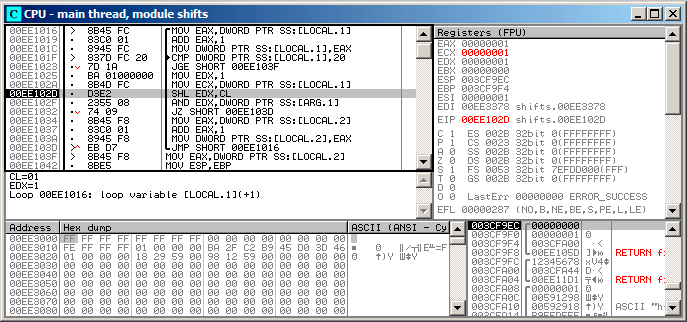
\includegraphics[scale=\FigScale]{patterns/14_bitfields/4_popcnt/olly1_1.png}
\caption{\olly: $i=1$, $i$ \RU{загружено в}\EN{is loaded into} \ECX}
\label{fig:shifts_olly1_1}
\end{figure}

\EDX \RU{содержит}\EN{is} $1$. \RU{Сейчас будет исполнена }\TT{SHL}\EN{ is to be executed now}.

\clearpage
\TT{SHL} \RU{исполнилась}\EN{was executed}:

\begin{figure}[H]
\centering
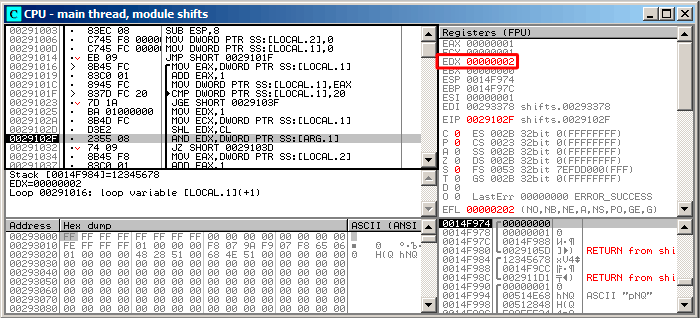
\includegraphics[scale=\FigScale]{patterns/14_bitfields/4_popcnt/olly1_2.png}
\caption{\olly: $i=1$, \EDX=$1 \ll 1=2$}
\label{fig:shifts_olly1_2}
\end{figure}

\EDX \RU{содержит}\EN{contain} $1 \ll 1$ (\OrENRU $2$). \RU{Это битовая маска}\EN{This is a bit mask}.

\clearpage
\ANDIns \RU{устанавливает}\EN{sets} \ZF \RU{в}\EN{to} $1$, 
\RU{что означает, что входное значение}\EN{which is meaning that input value} (\TT{0x12345678}) 
\RU{умножается\footnote{Логическое ``И''} с}\EN{ ANDed with} $2$ \RU{давая в результате}\EN{resulting} $0$:

\begin{figure}[H]
\centering
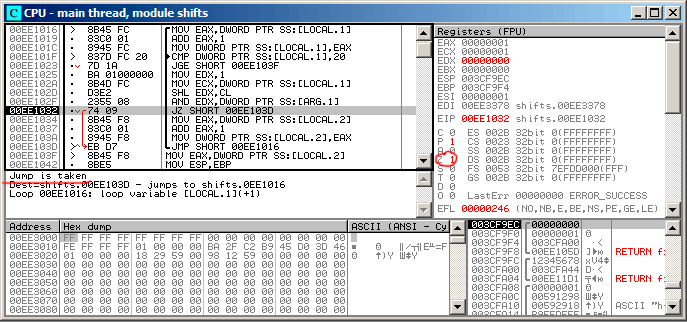
\includegraphics[scale=\FigScale]{patterns/14_bitfields/4_popcnt/olly1_3.png}
\caption{\olly: $i=1$, \RU{есть ли этот бит во входном значении? Нет.}
\EN{are there that bit in the input value? No.} (\ZF=1)}
\label{fig:shifts_olly1_3}
\end{figure}

\RU{Так что, во входном значении соответствующего бита нет}\EN{So, there are no corresponding bit in input value}.
\RU{Участок кода, увеличивающий счетчик бит на единицу не будет исполнен: инструкция \JZ \textit{обойдет} его}
\EN{The piece of code, which \glslink{increment}{increments} counter will not be executed: 
\JZ instruction will \textit{bypass} it}.

\clearpage
\RU{Я немного потрассировал далее и}\EN{Now I traced some time further and} $i$ \RU{теперь}\EN{is now} $4$.
\TT{SHL} \RU{исполнилась}\EN{is to be executed now}:

\begin{figure}[H]
\centering
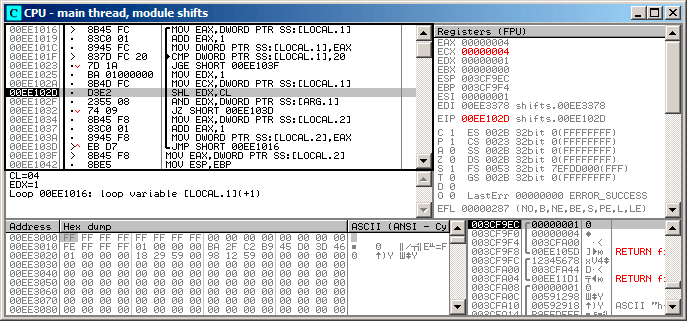
\includegraphics[scale=\FigScale]{patterns/14_bitfields/4_popcnt/olly4_1.png}
\caption{\olly: $i=4$, $i$ \RU{загружено в}\EN{is loaded into} \ECX}
\label{fig:shifts_olly4_1}
\end{figure}

\clearpage
\EDX=$1 \ll 4$ (\OrENRU \TT{0x10} \OrENRU $16$): 

\begin{figure}[H]
\centering
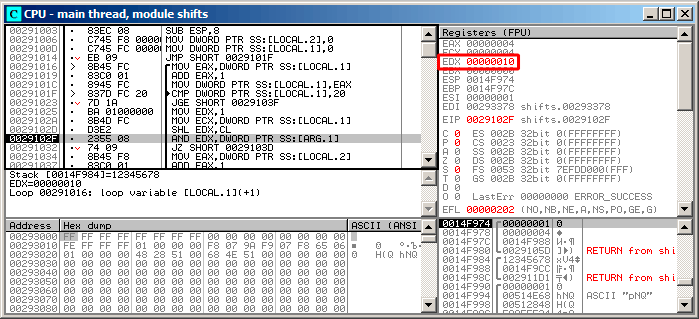
\includegraphics[scale=\FigScale]{patterns/14_bitfields/4_popcnt/olly4_2.png}
\caption{\olly: $i=4$, \EDX=$1 \ll 4=0x10$}
\label{fig:shifts_olly4_2}
\end{figure}

\RU{Это еще одна битовая маска}\EN{This is another bit mask}.

\clearpage
\ANDIns \RU{исполнилась}\EN{is executed}:

\begin{figure}[H]
\centering
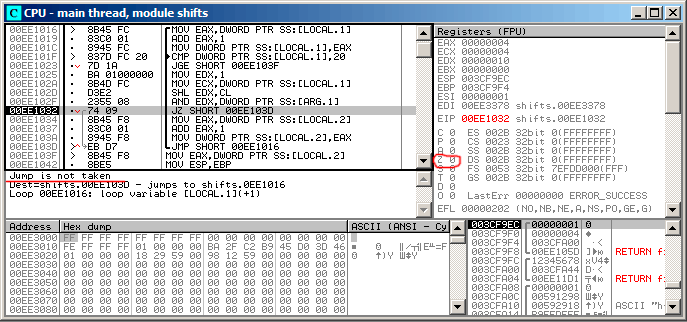
\includegraphics[scale=\FigScale]{patterns/14_bitfields/4_popcnt/olly4_3.png}
\caption{\olly: $i=4$, \RU{есть ли этот бит во входном значении? Да.}
\EN{are there that bit in the input value? Yes.} (\ZF=0)}
\label{fig:shifts_olly4_3}
\end{figure}

\ZF \RU{сейчас}\EN{is} $0$ \RU{потому что этот бит присутствует во входном значении}
\EN{because this bit is present in input value}.
\RU{Действительно}\EN{Indeed}, \TT{0x12345678 \& 0x10 = 0x10}. 
\RU{Этот бит считается: переход не сработает и счетчик бит будет увеличен на единицу}\EN{This bit counts: 
jump will not trigger and bits counter will be \glslink{increment}{incremented} now}.\\
\\
\RU{Ф-ция возвращает}\EN{The function returns} $13$. 
\RU{Это количество установленных бит в значении}\EN{This is total bits set in} \TT{0x12345678}\EN{ value}.


\subsubsection{GCC}

\RU{Скомпилируем то же и в}\EN{Let's compile it in} GCC 4.4.1:

\lstinputlisting[caption=GCC 4.4.1]{patterns/14_bitfields/4_popcnt/shifts_gcc.asm}

\subsection{x64}
\label{subsec:popcnt}

\RU{Я немного изменли пример, расширив его до 64-х бит}\EN{I modified the example slightly to extend it to 64-bit}:

\lstinputlisting[label=popcnt_x64_example]{patterns/14_bitfields/4_popcnt/shifts64.c}

\subsubsection{\NonOptimizing GCC 4.8.2}

\RU{Пока всё просто}\EN{So far so easy}.

\lstinputlisting[caption=\NonOptimizing GCC 4.8.2]{patterns/14_bitfields/4_popcnt/shifts64_GCC_O0.s.\LANG}

\subsubsection{\Optimizing GCC 4.8.2}

\lstinputlisting[caption=\Optimizing GCC 4.8.2,numbers=left,label=shifts64_GCC_O3]{patterns/14_bitfields/4_popcnt/shifts64_GCC_O3.s.\LANG}

\RU{Код более лаконичный, но содержит одну необычную вещь}\EN{This code is terser, but has a quirk}.
\RU{Во всех примерах, что мы пока видели, инкремент значения переменной ``rt'' происходит после сравнения 
определенного бита с единицей, но здесь ``rt'' увеличивается на 1 до этого (строка 6), записывая новое значение
в регистр \EDX.}
\EN{In all examples that we see so far, we were incrementing the ``rt'' value after comparing a specific bit,
but the code here increments ``rt'' before (line 6), writing the new value into register \EDX .}
\RU{Затем, если последний бит был 1, инструкция}\EN{Thus, if the last bit is 1, the} \TT{CMOVNE}
\footnote{Conditional MOVe if Not Equal\RU{ (MOV если не равно)}}\EN{ instruction} 
(\RU{которая синонимична}\EN{which is a synonym for} \TT{CMOVNZ}
\footnote{Conditional MOVe if Not Zero\RU{ (MOV если не ноль)}}) \IT{\RU{фиксирует}\EN{commits}} 
\RU{новое значение}\EN{the new value of} ``rt''
\RU{копируя значение из}\EN{by moving} \EDX (``\RU{предполагаемое значение rt}\EN{proposed rt value}'') 
\RU{в}\EN{into} \EAX 
(``\RU{текущее}\EN{current} rt'' \RU{которое будет возвращено в конце ф-ции}\EN{to be returned at the end}).
\RU{Следовательно, инкремент происходит на каждом шаге цикла, т.е., 64 раза, вне всякой связи с входным
значением.}
\EN{Hence, the incrementing is done at each step of loop, i.e., 64 times, without any relation to the input value.}

\RU{Преимущество этого кода в том, что он содержит только один условный переход (в конце цикла) вместо
двух (пропускающий инкремент ``rt'' и еще один в конце цикла).}
\EN{The advantage of this code is that it contain only one conditional jump (at the end of the loop) instead of 
two jumps (skipping the ``rt'' value increment and at the end of loop).}
\RU{И это может работать быстрее на современных CPU с предсказателем переходов}
\EN{And that might work faster on the modern CPUs with branch predictors}: \ref{branch_predictors}.

\label{FATRET}
\index{x86!\Instructions!FATRET}
\RU{Последняя инструкция это}\EN{The last instruction is} \TT{REP RET} (\EN{opcode}\RU{опкод} \TT{F3 C3}) 
\RU{которая также называется}\EN{which is also called} \TT{FATRET} \RU{в}\EN{by} MSVC.
\RU{Это оптимизированная версия \RET, рекомендуемая AMD для вставки в конце ф-ции, если \RET идет
прямо после условного перехода}\EN{This is somewhat optimized version of \RET, 
which is recommended by AMD to be placed at the end of function, if \RET goes right after conditional jump}: 
\cite[p.15]{AMDOptimization}
\footnote{\RU{Больше об этом}\EN{More information on it}: \url{http://go.yurichev.com/17328}}.

\subsubsection{\Optimizing MSVC 2010}

\lstinputlisting[caption=MSVC 2010]{patterns/14_bitfields/4_popcnt/MSVC_2010_x64_Ox.asm.\LANG}

\index{x86!\Instructions!ROL}
\RU{Здесь используется инструкция}\EN{Here the} \TT{ROL} \RU{вместо}\EN{instruction is used instead of} 
\TT{SHL}, \RU{которая на самом деле}\EN{which is in fact} ``rotate left''\RU{ (прокручивать влево)} 
\RU{вместо}\EN{instead of} ``shift left''\RU{ (сдвиг влево)},
\RU{но здесь, в этом примере, она работает так же как и}\EN{but in this example 
it will work just as} \TT{SHL}.

\RU{Об этих ``прокручивающих'' инструкциях больше читайте здесь}\EN{You can read more about the rotate instruction 
here}: \ref{ROL_ROR}.

\Reg{8} \RU{здесь считает от 64 до 0}\EN{here is counting from 64 to 0}. 
\RU{Это как бы инвертированная переменная $i$}\EN{It's just like an inverted $i$}.

\RU{Вот таблица некоторых регистров в процессе исполнения}\EN{Here is a table of some registers during the execution}:

\begin{center}
\begin{tabular}{ | l | l | }
\hline
\cellcolor{blue!25} RDX & \cellcolor{blue!25} R8 \\
\hline
0x0000000000000001 & 64 \\
\hline
0x0000000000000002 & 63 \\
\hline
0x0000000000000004 & 62 \\
\hline
0x0000000000000008 & 61 \\
\hline
... & ... \\
\hline
0x4000000000000000 & 2 \\
\hline
0x8000000000000000 & 1 \\
\hline
\end{tabular}
\end{center}

\index{x86!\Instructions!FATRET}
\RU{В конце видим инструкцию}\EN{At the end we see the} \TT{FATRET}\RU{, которая была описана здесь}\EN{ instruction, 
which was explained here}: \ref{FATRET}.

\subsubsection{\Optimizing MSVC 2012}

\lstinputlisting[caption=MSVC 2012]{patterns/14_bitfields/4_popcnt/MSVC_2012_x64_Ox.asm.\LANG}

\index{\CompilerAnomaly}
\label{MSVC2012_anomaly}
\Optimizing MSVC 2012 \RU{делает почти то же самое что и оптимизирующий}\EN{does almost the same job as 
optimizing} MSVC 2010, \RU{но почему-то, он генерирует 2 идентичных тела цикла и счетчик цикла теперь 32
вместо 64}\EN{but somehow, it generates two identical loop bodies and the loop count is now 32 instead of 64}.
\RU{Честно говоря, я не знаю, почему. Какой-то трюк с оптимизацией? Может быть, телу цикла лучше быть
немного длиннее?}
\EN{To be honest, I don't know why. Some optimization trick? Maybe it's better for the loop body to be slightly 
longer?}
\RU{Так или иначе, я сознательно добавляю такой код здесь чтобы показать, что результат компилятора
иногда может быть очень странный и нелогичный, но прекрасно работающий, конечно же.}
\EN{Anyway, I have added the code here intentionally to show that sometimes the compiler output may be really weird and 
illogical, but perfectly working.}

\ifdefined\IncludeARM
\subsection{ARM + \OptimizingXcodeIV (\ARMMode)}

\lstinputlisting[caption=\OptimizingXcodeIV (\ARMMode),label=ARM_leaf_example4]{patterns/14_bitfields/4_popcnt/ARM_Xcode_O3.lst.\LANG}

\index{ARM!\Instructions!TST}
\TT{TST} \RU{это то же что и}\EN{is the same things as} \TEST \InENRU x86.

\index{ARM!Optional operators!LSL}
\index{ARM!Optional operators!LSR}
\index{ARM!Optional operators!ASR}
\index{ARM!Optional operators!ROR}
\index{ARM!Optional operators!RRX}
\index{ARM!\Instructions!MOV}
\index{ARM!\Instructions!TST}
\index{ARM!\Instructions!CMP}
\index{ARM!\Instructions!ADD}
\index{ARM!\Instructions!SUB}
\index{ARM!\Instructions!RSB}
\RU{Как я уже указывал}\EN{As I mentioned before}~(\myref{shifts_in_ARM_mode}),
\RU{в режиме ARM нет отдельной инструкции для сдвигов.}
\EN{there are no separate shifting instructions in ARM mode.}
\RU{Однако, модификаторами}\EN{However, there are modifiers} 
LSL (\IT{Logical Shift Left}), 
LSR (\IT{Logical Shift Right}), 
ASR (\IT{Arithmetic Shift Right}), 
ROR (\IT{Rotate Right}) \AndENRU 
RRX (\IT{Rotate Right with Extend}) \RU{можно дополнять некоторые инструкции, такие как}
\EN{, which may be added to such instructions as} \MOV, \TT{TST},
\CMP, \ADD, \SUB, \TT{RSB}\footnote{\DataProcessingInstructionsFootNote}.

\RU{Эти модификаторы указывают, как сдвигать второй операнд, и на сколько.}
\EN{These modificators define how to shift the second operand and by how many bits.}

\index{ARM!\Instructions!TST}
\index{ARM!Optional operators!LSL}
\RU{Таким образом, инструкция }\EN{Thus the} \TT{``TST R1, R2,LSL R3''} 
\RU{здесь работает как}\EN{instruction works here as} $R1 \land (R2 \ll R3)$.

\subsection{ARM + \OptimizingXcodeIV (\ThumbTwoMode)}

\index{ARM!\Instructions!LSL.W}
\index{ARM!\Instructions!LSL}
\RU{Почти такое же}\EN{Almost the same}, 
\RU{только здесь применяется пара инструкций}\EN{but here are two} 
\TT{LSL.W}/\TT{TST} 
\RU{вместо одной}\EN{instructions are used instead of a single} 
\TT{TST},
\RU{ведь в режиме thumb нельзя добавлять указывать модификатор}\EN{because in thumb mode it is not
possible to define} \TT{LSL} \RU{прямо в}\EN{modifier directly in} \TT{TST}.

\begin{lstlisting}[label=ARM_leaf_example5]
                MOV             R1, R0
                MOVS            R0, #0
                MOV.W           R9, #1
                MOVS            R3, #0
loc_2F7A
                LSL.W           R2, R9, R3
                TST             R2, R1
                ADD.W           R3, R3, #1
                IT NE
                ADDNE           R0, #1
                CMP             R3, #32
                BNE             loc_2F7A
                BX              LR
\end{lstlisting}

\subsection{ARM64 + \Optimizing GCC 4.9}

\RU{Я взял 64-битный пример, который уже использовал}\EN{I took the 64-bit example I already used}: 
\myref{popcnt_x64_example}.

\lstinputlisting[caption=\Optimizing GCC (Linaro) 4.8]{patterns/14_bitfields/4_popcnt/ARM64_GCC_O3.s.\LANG}

\RU{Результат очень похож на тот, что GCC сгенерировал для x64}\EN{The result is very similar to what GCC 
generates for x64}: \myref{shifts64_GCC_O3}.

\index{ARM!\Instructions!CSEL}
\EN{The}\RU{Инструкция} \TT{CSEL} \RU{это}\EN{instruction is} ``Conditional SELect''\RU{ (выбор при условии)}, 
\RU{она просто выбирает одну из переменных, в зависимости от флагов выставленных}\EN{it just choose one 
variable of two depending on the flags set by} \TT{TST} \RU{и копирует значение в регистр}\EN{and copies the value 
into} \RegW{2}\RU{, содержащий переменную ``rt''}\EN{ , which holds the ``rt'' variable}.

\subsection{ARM64 + \NonOptimizing GCC 4.9}

\RU{И снова, я использовал 64-битный пример, который я уже использовал раннее}\EN{And again, the 64-bit 
example I already used}: \myref{popcnt_x64_example}.

\RU{Код более многословный, как обычно}\EN{The code is more verbose, as usual}.

\lstinputlisting[caption=\NonOptimizing GCC (Linaro) 4.8]{patterns/14_bitfields/4_popcnt/ARM64_GCC_O0.s.\LANG}

\fi
\ifdefined\IncludeMIPS
\subsection{MIPS}

\subsubsection{\NonOptimizing GCC}

\lstinputlisting[caption=\NonOptimizing GCC 4.4.5 (IDA)]{patterns/14_bitfields/4_popcnt/MIPS_O0_IDA.lst.\LANG}

\index{MIPS!\Instructions!SLL}
\index{MIPS!\Instructions!SLLV}
\RU{Это многословно: все локальные переменные расположены в локальном стеке и перезагружаются каждый раз,
когда нужны.}
\EN{That is verbose: all local variables are located in the local stack and reloaded each time they're needed.}
\RU{Инструкция SLLV это \q{Shift Word Left Logical Variable}, она отличается от SLL только тем что
количество бит для сдвига кодируется в SLL (и, следовательно, фиксировано), а SLL берет количество из регистра.}
\EN{The SLLV instruction is \q{Shift Word Left Logical Variable}, it differs from SLL only in that
the shift amount is encoded in the SLL instruction (and is fixed, as a consequence), 
but SLLV takes shift amount from a register.}

\subsubsection{\Optimizing GCC}

\RU{Это более сжато}\EN{That is terser}.
\RU{Здесь две инструкции сдвигов вместо одной.}\EN{There are two shift instructions instead of one.}
\RU{Почему}\EN{Why}?
\RU{Можно заменить первую инструкцию SLLV на инструкцию безусловного перехода, передав управление прямо
на вторую SLLV.}
\EN{It's possible to replace the first SLLV instruction with an unconditional branch instruction that 
jumps right to the second SLLV.}
\RU{Но это еще одна инструкция перехода в функции, а от них избавляться всегда выгодно}
\EN{But this is another branching instruction in the function, and it's always favorable to get rid of them}: 
\myref{branch_predictors}.

\lstinputlisting[caption=\Optimizing GCC 4.4.5 (IDA)]{patterns/14_bitfields/4_popcnt/MIPS_O3_IDA.lst.\LANG}

\fi

% TODO: add ROL/ROR
\section{\Conclusion{}}

\index{x86!\Instructions!SHR}
\index{x86!\Instructions!SHL}
\index{x86!\Instructions!SAR}
\RU{Инструкции сдвига, аналогичные операторам \CCpp $\ll$ и $\gg$, в x86 это SHR/SHL (для беззнаковых значений),
SAR/SHL (для знаковых значений).}
\EN{Analogous to the \CCpp shifting operators $\ll$ and $\gg$, 
the shift instructions in x86 are SHR/SHL (for unsigned values) and SAR/SHL (for signed values).}

\index{ARM!\Instructions!LSR}
\index{ARM!\Instructions!LSL}
\index{ARM!\Instructions!ASR}
\RU{Инструкции сдвига в ARM это LSR/LSL (для беззнаковых значений), ASR/LSL (для знаковых значений).}
\EN{The shift instructions in ARM are LSR/LSL (for unsigned values) and ASR/LSL (for signed values).}
\RU{Можно также добавлять суффикс сдвига для некоторых инструкций 
(которые называются \q{data processing instructions}).}
\EN{It's also possible to add shift suffix to some instructions 
(which are called \q{data processing instructions}).}
% FIXME: which instructions?

\subsection{\RU{Проверка определенного бита (известного на стадии компиляции)}
\EN{Check for specific bit (known at compile stage)}}

\RU{Проверить, присутствует ли бит 1000000 (0x40) в значении в регистре:}
\EN{Test if the 1000000 bit (0x40) is present in the register's value:}

\lstinputlisting[caption=\CCpp]{patterns/14_bitfields/c_snippet0.c}

\lstinputlisting[caption=x86]{patterns/14_bitfields/TEST_JNZ.lst.\LANG}

\lstinputlisting[caption=x86]{patterns/14_bitfields/TEST_JZ.lst.\LANG}

\ifdefined\IncludeARM
\lstinputlisting[caption=ARM (\ARMMode)]{patterns/14_bitfields/TST_BNE.lst.\LANG}
\fi

\index{x86!\Instructions!AND}
\index{x86!\Instructions!TEST}
\RU{Иногда AND используется вместо TEST, но флаги выставляются точно также.}
\EN{Sometimes, AND is used instead of TEST, but the flags that are set are the same.}

\subsection{\RU{Проверка определенного бита (заданного во время исполнения)}
\EN{Check for specific bit (specified at runtime)}}

\RU{Это обычно происходит при помощи вот такого фрагмента на \CCpp (сдвинуть значение на $n$ бит вправо,
затем отрезать самый младший бит):}
\EN{This is usually done by this \CCpp code snippet (shift value by $n$ bits right, then cut off lowest bit):}

\lstinputlisting[caption=\CCpp]{patterns/14_bitfields/c_snippet1.c}

\RU{Это обычно реализуется в x86-коде так:}
\EN{This is usually implemented in x86 code as:}

\begin{lstlisting}[caption=x86]
; REG=input_value
; CL=n
SHR REG, CL
AND REG, 1
\end{lstlisting}

\RU{Или (сдвинуть $1$ $n$ раз влево, изолировать этот же бит во входном значении и проверить, не ноль ли он):}
\EN{Or (shift $1$ bit $n$ times left, isolate this bit in input value and check if it's not zero):}

\lstinputlisting[caption=\CCpp]{patterns/14_bitfields/c_snippet2.c}

\RU{Это обычно так реализуется в x86-коде:}
\EN{This is usually implemented in x86 code as:}

\begin{lstlisting}[caption=x86]
; CL=n
MOV REG, 1
SHL REG, CL
AND input_value, REG
\end{lstlisting}

\subsection{\RU{Установка определенного бита (известного во время компиляции)}
\EN{Set specific bit (known at compile stage)}}

\begin{lstlisting}[caption=\CCpp]
value=value|0x40;
\end{lstlisting}

\begin{lstlisting}[caption=x86]
OR REG, 40h
\end{lstlisting}

\ifdefined\IncludeARM
\begin{lstlisting}[caption=ARM (\ARMMode) \AndENRU ARM64]
ORR R0, R0, #0x40
\end{lstlisting}
\fi

\subsection{\RU{Установка определенного бита (заданного во время исполнения)}
\EN{Set specific bit (specified at runtime)}}

\lstinputlisting[caption=\CCpp]{patterns/14_bitfields/c_snippet3.c}

\RU{Это обычно так реализуется в x86-коде:}
\EN{This is usually implemented in x86 code as:}

\begin{lstlisting}[caption=x86]
; CL=n
MOV REG, 1
SHL REG, CL
OR input_value, REG
\end{lstlisting}

\subsection{\RU{Сброс определенного бита (известного во время компиляции)}
\EN{Clear specific bit (known at compile stage)}}

\RU{Просто исполните операцию логического \q{И} (AND) с инвертированным значением:}
\EN{Just apply AND operation with the inverted value:}

\begin{lstlisting}[caption=\CCpp]
value=value&(~0x40);
\end{lstlisting}

\begin{lstlisting}[caption=x86]
AND REG, 0FFFFFFBFh
\end{lstlisting}

\begin{lstlisting}[caption=x64]
AND REG, 0FFFFFFFFFFFFFFBFh
\end{lstlisting}

\RU{Это на самом деле сохранение всех бит кроме одного.}
\EN{This is actually leaving all bits set except one.}

\ifdefined\IncludeARM
\index{ARM!\Instructions!BIC}
\RU{В ARM в режиме ARM есть инструкция BIC, работающая как две инструкции NOT+AND:}
\EN{ARM in ARM mode has BIC instruction, which works like the NOT+AND instruction pair:}

\begin{lstlisting}[caption=ARM (\ARMMode)]
BIC R0, R0, #0x40
\end{lstlisting}
\fi

\subsection{\RU{Сброс определенного бита (заданного во время исполнения)}
\EN{Clear specific bit (specified at runtime)}}

\lstinputlisting[caption=\CCpp]{patterns/14_bitfields/c_snippet4.c}

\begin{lstlisting}[caption=x86]
; CL=n
MOV REG, 1
SHL REG, CL
NOT REG
AND input_value, REG
\end{lstlisting}

\ifdefined\IncludeExercises
\section{\Exercises}

\subsection{\Exercise \#1}
\label{exercise_bitfields_1}

\WhatThisCodeDoes\

\begin{lstlisting}[caption=\Optimizing MSVC 2010]
_a$ = 8
_f	PROC
	mov	ecx, DWORD PTR _a$[esp-4]
	mov	eax, ecx
	mov	edx, ecx
	shl	edx, 16		; 00000010H
	and	eax, 65280	; 0000ff00H
	or	eax, edx
	mov	edx, ecx
	and	edx, 16711680	; 00ff0000H
	shr	ecx, 16		; 00000010H
	or	edx, ecx
	shl	eax, 8
	shr	edx, 8
	or	eax, edx
	ret	0
_f	ENDP
\end{lstlisting}

\begin{lstlisting}[caption=\OptimizingKeilVI (\ARMMode)]
f PROC
        MOV      r1,#0xff0000
        AND      r1,r1,r0,LSL #8
        MOV      r2,#0xff00
        ORR      r1,r1,r0,LSR #24
        AND      r2,r2,r0,LSR #8
        ORR      r1,r1,r2
        ORR      r0,r1,r0,LSL #24
        BX       lr
        ENDP
\end{lstlisting}

\begin{lstlisting}[caption=\OptimizingKeilVI (\ThumbMode)]
f PROC
        MOVS     r3,#0xff
        LSLS     r2,r0,#8
        LSLS     r3,r3,#16
        ANDS     r2,r2,r3
        LSRS     r1,r0,#24
        ORRS     r1,r1,r2
        LSRS     r2,r0,#8
        ASRS     r3,r3,#8
        ANDS     r2,r2,r3
        ORRS     r1,r1,r2
        LSLS     r0,r0,#24
        ORRS     r0,r0,r1
        BX       lr
        ENDP
\end{lstlisting}

\begin{lstlisting}[caption=\Optimizing GCC 4.9 (ARM64)]
f:
	rev	w0, w0
	ret
\end{lstlisting}

\lstinputlisting[caption=\Optimizing GCC 4.4.5 (MIPS) (IDA)]{patterns/14_bitfields/1_MIPS_O3_IDA.lst}

\Answer{}: \ref{exercise_solutions_bitfields_1}.

\subsection{\Exercise \#2}
\label{exercise_bitfields_2}

\WhatThisCodeDoes\

\begin{lstlisting}[caption=\Optimizing MSVC 2010]
_a$ = 8							; size = 4
_f	PROC
	push	esi
	mov	esi, DWORD PTR _a$[esp]
	xor	ecx, ecx
	push	edi
	lea	edx, DWORD PTR [ecx+1]
	xor	eax, eax
	npad	3 ; align next label
$LL3@f:
	mov	edi, esi
	shr	edi, cl
	add	ecx, 4
	and	edi, 15
	imul	edi, edx
	lea	edx, DWORD PTR [edx+edx*4]
	add	eax, edi
	add	edx, edx
	cmp	ecx, 28
	jle	SHORT $LL3@f
	pop	edi
	pop	esi
	ret	0
_f	ENDP
\end{lstlisting}

\begin{lstlisting}[caption=\OptimizingKeilVI (\ARMMode)]
f PROC
        MOV      r3,r0
        MOV      r1,#0
        MOV      r2,#1
        MOV      r0,r1
|L0.16|
        LSR      r12,r3,r1
        AND      r12,r12,#0xf
        MLA      r0,r12,r2,r0
        ADD      r1,r1,#4
        ADD      r2,r2,r2,LSL #2
        CMP      r1,#0x1c
        LSL      r2,r2,#1
        BLE      |L0.16|
        BX       lr
        ENDP
\end{lstlisting}

\begin{lstlisting}[caption=\OptimizingKeilVI (\ThumbMode)]
f PROC
        PUSH     {r4,lr}
        MOVS     r3,r0
        MOVS     r1,#0
        MOVS     r2,#1
        MOVS     r0,r1
|L0.10|
        MOVS     r4,r3
        LSRS     r4,r4,r1
        LSLS     r4,r4,#28
        LSRS     r4,r4,#28
        MULS     r4,r2,r4
        ADDS     r0,r4,r0
        MOVS     r4,#0xa
        MULS     r2,r4,r2
        ADDS     r1,r1,#4
        CMP      r1,#0x1c
        BLE      |L0.10|
        POP      {r4,pc}
        ENDP
\end{lstlisting}

\begin{lstlisting}[caption=\NonOptimizing GCC 4.9 (ARM64)]
f:
	sub	sp, sp, #32
	str	w0, [sp,12]
	str	wzr, [sp,28]
	mov	w0, 1
	str	w0, [sp,24]
	str	wzr, [sp,20]
	b	.L2
.L3:
	ldr	w0, [sp,28]
	ldr	w1, [sp,12]
	lsr	w0, w1, w0
	and	w1, w0, 15
	ldr	w0, [sp,24]
	mul	w0, w1, w0
	ldr	w1, [sp,20]
	add	w0, w1, w0
	str	w0, [sp,20]
	ldr	w0, [sp,28]
	add	w0, w0, 4
	str	w0, [sp,28]
	ldr	w1, [sp,24]
	mov	w0, w1
	lsl	w0, w0, 2
	add	w0, w0, w1
	lsl	w0, w0, 1
	str	w0, [sp,24]
.L2:
	ldr	w0, [sp,28]
	cmp	w0, 28
	ble	.L3
	ldr	w0, [sp,20]
	add	sp, sp, 32
	ret
\end{lstlisting}

\lstinputlisting[caption=\Optimizing GCC 4.4.5 (MIPS) (IDA)]{patterns/14_bitfields/2_MIPS_O3_IDA.lst}

\Answer{}: \ref{exercise_solutions_bitfields_2}.

\subsection{\Exercise \#3}
\label{exercise_bitfields_3}

\EN{Using \ac{MSDN} documentation, find out, which flags were used in \TT{MessageBox()} win32 function call.}
\RU{Используя документацию \ac{MSDN}, найдите, какие флаги использовались в вызове win32-функции 
\TT{MessageBox()}.}

\begin{lstlisting}[caption=\Optimizing MSVC 2010]
_main	PROC
	push	278595		; 00044043H
	push	OFFSET $SG79792 ; 'caption'
	push	OFFSET $SG79793 ; 'hello, world!'
	push	0
	call	DWORD PTR __imp__MessageBoxA@16
	xor	eax, eax
	ret	0
_main	ENDP
\end{lstlisting}

\Answer{}: \ref{exercise_solutions_bitfields_3}.

\subsection{\Exercise \#4}
\label{exercise_bitfields_4}

\WhatThisCodeDoes\

\begin{lstlisting}[caption=\Optimizing MSVC 2010]
_m$ = 8		; size = 4
_n$ = 12	; size = 4
_f	PROC
	mov	ecx, DWORD PTR _n$[esp-4]
	xor	eax, eax
	xor	edx, edx
	test	ecx, ecx
	je	SHORT $LN2@f
	push	esi
	mov	esi, DWORD PTR _m$[esp]
$LL3@f:
	test	cl, 1
	je	SHORT $LN1@f
	add	eax, esi
	adc	edx, 0
$LN1@f:
	add	esi, esi
	shr	ecx, 1
	jne	SHORT $LL3@f
	pop	esi
$LN2@f:
	ret	0
_f	ENDP
\end{lstlisting}

\begin{lstlisting}[caption=\OptimizingKeilVI (\ARMMode)]
f PROC
        PUSH     {r4,lr}
        MOV      r3,r0
        MOV      r0,#0
        MOV      r2,r0
        MOV      r12,r0
        B        |L0.48|
|L0.24|
        TST      r1,#1
        BEQ      |L0.40|
        ADDS     r0,r0,r3
        ADC      r2,r2,r12
|L0.40|
        LSL      r3,r3,#1
        LSR      r1,r1,#1
|L0.48|
        CMP      r1,#0
        MOVEQ    r1,r2
        BNE      |L0.24|
        POP      {r4,pc}
        ENDP
\end{lstlisting}

\begin{lstlisting}[caption=\OptimizingKeilVI (\ThumbMode)]
f PROC
        PUSH     {r4,r5,lr}
        MOVS     r3,r0
        MOVS     r0,#0
        MOVS     r2,r0
        MOVS     r4,r0
        B        |L0.24|
|L0.12|
        LSLS     r5,r1,#31
        BEQ      |L0.20|
        ADDS     r0,r0,r3
        ADCS     r2,r2,r4
|L0.20|
        LSLS     r3,r3,#1
        LSRS     r1,r1,#1
|L0.24|
        CMP      r1,#0
        BNE      |L0.12|
        MOVS     r1,r2
        POP      {r4,r5,pc}
        ENDP
\end{lstlisting}

\begin{lstlisting}[caption=\Optimizing GCC 4.9 (ARM64)]
f:
	mov	w2, w0
	mov	x0, 0
	cbz	w1, .L2
.L3:
	and	w3, w1, 1
	lsr	w1, w1, 1
	cmp	w3, wzr
	add	x3, x0, x2, uxtw
	lsl	w2, w2, 1
	csel	x0, x3, x0, ne
	cbnz	w1, .L3
.L2:
	ret
\end{lstlisting}

\lstinputlisting[caption=\Optimizing GCC 4.4.5 (MIPS) (IDA)]{patterns/14_bitfields/4_MIPS_O3_IDA.lst}

\Answer{}: \ref{exercise_solutions_bitfields_4}.

\fi
